%% Adaptado a partir de :
%%    abtex2-modelo-trabalho-academico.tex, v-1.9.2 laurocesar
%% para ser um modelo para os trabalhos no IFSP-SPO

\documentclass[
    % -- opções da classe memoir --
    12pt,               % tamanho da fonte
    openright,          % capítulos começam em pág ímpar (insere página vazia caso preciso)
    %twoside,            % para impressão em verso e anverso. Oposto a oneside
    oneside,
    a4paper,            % tamanho do papel. 
    % -- opções da classe abntex2 --schwinn
    % Opções que não devem ser utilizadas na versão final do documento
    %draft,              % para compilar mais rápido, remover na versão final
    MODELO,             % indica que é um documento modelo então precisa dos geradores de texto
    TODO,               % indica que deve apresentar lista de pendencias 
    % -- opções do pacote babel --
    english,            % idioma adicional para hifenização
    brazil              % o último idioma é o principal do documento
    ]{ifsp-spo-inf-ctds} % ajustar de acordo com o modelo desejado para o curso

% ---
% Pacotes básicos 
% ---
%\usepackage[utf8]{inputenc}     % Codificacao do documento (conversão automática dos acentos)
% ---

%\usepackage{style}
        

% --- 
% CONFIGURAÇÕES DE PACOTES ADICIONAIS UTEIS
% --- 


% ---
% Informações de dados para CAPA e FOLHA DE ROSTO
% ---
\titulo{DowJonesSkins}

% Trabalho individual
%\autor{AUTOR DO TRABALHO}

% Trabalho em Equipe
% ver também https://github.com/abntex/abntex2/wiki/FAQ#como-adicionar-mais-de-um-autor-ao-meu-projeto
\renewcommand{\imprimirautor}{
\begin{tabular}{lr}
Andrey Camargo Lacerda &  SP3013049 \\
Fabricio Ernesto dos Santos & SP3013171 \\
Guilherme Oliveira de Souza Leão & SP3013243 \\
Luis Antonio Gonçalves Novaes Angelim & SP301309X \\
Vitor Urdiali da Silva &  SP3013111 \\
\end{tabular}
}


\disciplina{DW2A4 - Desenvolvimento Web II}
%\disciplina{MTPA4 - Metodologia da Pesquisa Científica}
%\disciplina{ES4A4 - Engenharia de Software IV}

\preambulo{Monografia do Projeto de DW2A4, MTPA4 e ESA4A orientadas pelos professores Luis Fernando Aires Branco Menegueti (DW2A4 e MTPA4) e
Daniel Marques Gomes de Morais(ES4A4).}

\data{22 de Novembro de 2019}

% Definir o que for necessário e comentar o que não for necessário
% Utilizar o Nome Completo, abntex tem orientador e coorientador
% então vão ser utilizados na definição de professor
\renewcommand{\orientadorname}{Professor:}
\orientador{Luis Fernando Aires Branco Menegueti}
\renewcommand{\coorientadorname}{Professor:}
\coorientador{Daniel Marques Gomes de Morais}


% ---


% informações do PDF
\makeatletter
\hypersetup{
        %pagebackref=true,
        pdftitle={\@title}, 
        pdfauthor={\@author},
        pdfsubject={\imprimirpreambulo},
        pdfcreator={LaTeX with abnTeX2 using IFSP model},
        pdfkeywords={abnt}{latex}{abntex}{abntex2}{IFSP}{\ifspprefixo}{trabalho acadêmico}, 
        colorlinks=true,            % false: boxed links; true: colored links
        linkcolor=blue,             % color of internal links
        citecolor=blue,             % color of links to bibliography
        filecolor=magenta,              % color of file links
        urlcolor=blue,
        bookmarksdepth=4
}
\makeatother
% --- 


% ----
% Início do documento
% ----
\begin{document}

% Retira espaço extra obsoleto entre as frases.
%\frenchspacing 

%somente para o exemplo, fica primeiro
%\newcommand{\urlmodelosimples}{https://www.sharelatex.com/project/58a3a66af9bb74023ba1bd56}

\newcommand{\urlmodelo}{\url{\urlmodelosimples}}

Esse documento foi feito a partir do modelo canônico do \abnTeX, o acesso ao PDF pode ser feito em 
\urlmodelo. A estrutura utilizada aqui foi um modelo utilizado no curso de Pós Graduação em Gestão de TI do \ac{ifsp}.
\todo{Remover texto informativo inicial}

%%A versão do sharelatex atualmente é a mais atualizada

%A versão atualizada da classe \ac{ifsp} para \LaTeX pode ser acessada em %\url{https://github.com/ivanfmartinez/latexlib/tree/master/ifsp}.

Este documento não pode ser considerado como um padrão a ser seguido em sua totalidade, ele tem como maior objetivo demonstrar como utilizar o \LaTeX\ para obter um documento atendendo ao máximo o padrão do \ac{ifsp} e \ac{abnt}.

Algumas bibliotecas \LaTeX\ disponíveis no overleaf estão desatualizadas, para melhores resultados é recomendável a utilização de outro compilador utilizando as ultimas versões de todas bibliotecas



\noindent\hrulefill



\newpage


% -- lista de pendencias gerada pelo todonotes
% -- altere opções do usepackage para remover na versão final....
%\listoftodos
\newpage

% ----------------------------------------------------------
% ELEMENTOS PRÉ-TEXTUAIS
% ----------------------------------------------------------
%\pretextual

% ---
% Capa
% ---
\imprimircapa

\newcounter{todocounter}
\newcommand{\todonum}[2][]
{\stepcounter{todocounter}\todo[#1]{\thetodocounter: #2}}


% ---

% ---
% Folha de rosto
% (o * indica que haverá a ficha bibliográfica)
% ---
\imprimirfolhaderosto
%\imprimirfolhaderosto*
% ---

% Quando registrado na biblioteca
%
% ---
% Inserir a ficha bibliografica
% ---

% Isto é um exemplo de Ficha Catalográfica, ou ``Dados internacionais de
% catalogação-na-publicação''. Você pode utilizar este modelo como referência. 
% Porém, provavelmente a biblioteca da sua universidade lhe fornecerá um PDF
% com a ficha catalográfica definitiva após a defesa do trabalho. Quando estiver
% com o documento, salve-o como PDF no diretório do seu projeto e substitua todo
% o conteúdo de implementação deste arquivo pelo comando abaixo:
%
% \begin{fichacatalografica}
%     \includepdf{fig_ficha_catalografica.pdf}
% \end{fichacatalografica}
\begin{fichacatalografica}
    \vspace*{\fill}                 % Posição vertical
    \hrule                          % Linha horizontal
    \begin{center}                  % Minipage Centralizado
    \begin{minipage}[c]{12.5cm}     % Largura
    
    \imprimirautor
    
    \hspace{0.5cm} \imprimirtitulo  / \imprimirautor. --
    \imprimirlocal, \imprimirdata-
    
    \hspace{0.5cm} \pageref{LastPage} p. : il. (algumas color.) ; 30 cm.\\
    
    \hspace{0.5cm} \imprimirorientadorRotulo~\imprimirorientador\\
    
    \hspace{0.5cm}
    \parbox[t]{\textwidth}{\imprimirtipotrabalho~--~\imprimirinstituicao,
    \imprimirdata.}\\
    
    \hspace{0.5cm}
        1. Palavra-chave1.
        2. Palavra-chave2.
        I. Orientador.
        II. Universidade xxx.
        III. Faculdade de xxx.
        IV. Título\\            
    
    \hspace{8.75cm} CDU 02:141:005.7\\
    
    \end{minipage}
    \end{center}
    \hrule
\end{fichacatalografica}
% ---



%Caso necessário
%% ---
% Inserir errata
% ---
\begin{errata}
Elemento opcional da \citeonline[4.2.1.2]{NBR14724:2011}. Exemplo:

\vspace{\onelineskip}


FERRIGNO, C. R. A. \textbf{Tratamento de neoplasias ósseas apendiculares com
reimplantação de enxerto ósseo autólogo autoclavado associado ao plasma
rico em plaquetas}: estudo crítico na cirurgia de preservação de membro em
cães. 2011. 128 f. Tese (Livre-Docência) - Faculdade de Medicina Veterinária e
Zootecnia, Universidade de São Paulo, São Paulo, 2011.

\begin{table}[htb]
\center
\footnotesize
\begin{tabular}{|p{1.4cm}|p{1cm}|p{3cm}|p{3cm}|}
  \hline
   \textbf{Folha} & \textbf{Linha}  & \textbf{Onde se lê}  & \textbf{Leia-se}  \\
    \hline
    1 & 10 & auto-conclavo & autoconclavo\\
   \hline
\end{tabular}
\end{table}

\end{errata}
% ---

%Obrigatório para trabalhos com bancas oficiais
%% ---
% Inserir folha de aprovação
% ---

% Isto é um exemplo de Folha de aprovação, elemento obrigatório da NBR
% 14724/2011 (seção 4.2.1.3). Você pode utilizar este modelo até a aprovação
% do trabalho. Após isso, substitua todo o conteúdo deste arquivo por uma
% imagem da página assinada pela banca com o comando abaixo:
%
% \includepdf{folhadeaprovacao_final.pdf}
%
\begin{folhadeaprovacao}

  \begin{center}
    {\ABNTEXchapterfont\large\imprimirautor}

    \vspace*{\fill}\vspace*{\fill}
    \begin{center}
      \ABNTEXchapterfont\bfseries\Large\imprimirtitulo
    \end{center}
    \vspace*{\fill}
    
    \hspace{.45\textwidth}
    \begin{minipage}{.5\textwidth}
        \imprimirpreambulo
    \end{minipage}%
    \vspace*{\fill}
   \end{center}
        
   Trabalho aprovado. \imprimirlocal, 24 de novembro de 2012:

   \assinatura{\textbf{\imprimirorientador} \\ Orientador} 
   \assinatura{\textbf{Professor} \\ Convidado 1}
   \assinatura{\textbf{Professor} \\ Convidado 2}
   %\assinatura{\textbf{Professor} \\ Convidado 3}
   %\assinatura{\textbf{Professor} \\ Convidado 4}
      
   \begin{center}
    \vspace*{0.5cm}
    {\large\imprimirlocal}
    \par
    {\large\imprimirdata}
    \vspace*{1cm}
  \end{center}
  
\end{folhadeaprovacao}
% ---


% ---- opcionais 
%% ---
% Dedicatória
% ---
\begin{dedicatoria}
   \vspace*{\fill}
   \centering
   \noindent
   \textit{ Este trabalho é dedicado às crianças adultas que,\\
   quando pequenas, sonharam em se tornar cientistas.} 

\todonum{colocar sua dedicatoria}
   
   \vspace*{\fill}
   

\end{dedicatoria}
% ---
%% ---
% Agradecimentos
% ---
\begin{agradecimentos}
\todonum{colocar seus agradecimentos}
Os agradecimentos principais são direcionados à Gerald Weber, Miguel Frasson,
Leslie H. Watter, Bruno Parente Lima, Flávio de Vasconcellos Corrêa, Otavio Real
Salvador, Renato Machnievscz\footnote{Os nomes dos integrantes do primeiro
projeto abn\TeX\ foram extraídos de
\url{http://codigolivre.org.br/projects/abntex/}} e todos aqueles que
contribuíram para que a produção de trabalhos acadêmicos conforme
as normas ABNT com \LaTeX\ fosse possível.

Agradecimentos especiais são direcionados ao Centro de Pesquisa em Arquitetura
da Informação\footnote{\url{http://www.cpai.unb.br/}} da Universidade de
Brasília (CPAI), ao grupo de usuários
\emph{latex-br}\footnote{\url{http://groups.google.com/group/latex-br}} e aos
novos voluntários do grupo
\emph{\abnTeX}\footnote{\url{http://groups.google.com/group/abntex2} e
\url{http://abntex2.googlecode.com/}}~que contribuíram e que ainda
contribuirão para a evolução do \abnTeX.

\end{agradecimentos}
% ---
%% ---
% Epígrafe
% ---
\begin{epigrafe}
    \vspace*{\fill}
    \begin{flushright}
        \textit{``Não vos amoldeis às estruturas deste mundo, \\
        mas transformai-vos pela renovação da mente, \\
        a fim de distinguir qual é a vontade de Deus: \\
        o que é bom, o que Lhe é agradável, o que é perfeito.\\
        (Bíblia Sagrada, Romanos 12, 2)}
    \end{flushright}
\end{epigrafe}
% ---

% -- resumo obrigatório
% ---
% RESUMOS
% ---

% resumo em português
\setlength{\absparsep}{18pt} % ajusta o espaçamento dos parágrafos do resumo
\begin{resumo}
Este trabalho de pesquisa visa a implementação de uma aplicação web que simule um
mercado financeiro para skins presentes no jogo eletrônico ``Counter-Strike: Global
Offensive'', funcionando como uma bolsa de valores e permitindo a modalidade de
negócio ``Day Trading''. Neste sistema, o usuário irá logar via Steam Account e
depositará suas skins no site, permitindo assim o investimento de suas skins, assim como
a compra de outras skins em investimento. O desenvolvimento e planejamento do
projeto beberá dos métodos ágeis, aplicando uma engenharia de software próxima ao
que reside na metodologia XP. Para isso a ferramenta Pivotal Tracker será utilizada
para administração do projeto, onde todas as Histórias de Usuário serão organizadas e
discutidas. Partindo para a parte mais técnica, o sistema será implementado utilizando
``HTML5'' para o front-end e ``Node.Js'' para o back-end. No back-end, o framework
``express'' será responsável por instanciar e administrar o servidores web. Para testes, os
frameworks ``Jest'' e ``Cucumber'' serão utilizados, enquanto para deploy e controle de
versão, o Heroku e o Github serão utilizados, respectivamente.


 \textbf{Palavras-chaves}:day trading de skins. bolsa de valores de skins. sistema de troca de
skins. aplicação web.
\end{resumo}

% resumo em inglês
\begin{resumo}[Abstract]
 \begin{otherlanguage*}{english}
%   This is the english abstract.
   \vspace{\onelineskip}

This research work aims at the implementation of a web application that simulates a
financial market for skins in the electronic game ``Counter-Strike: Global
Offensive'', functioning as a stock exchange and allowing the modality of
Day Trading business. In this system, the user will login via Steam Account and
deposit your skins on the site, allowing you to invest your skins as well as
buying other investment skins. The development and planning of the
project will drink from the applicable methods by applying software engineering
which lies in the XP methodology. For this the Pivotal Tracker tool will be used
for project administration, where all the ``User Stories'' will be organized and
discussed. Starting with the most technical part, the system will be implemented using
HTML5 for the front end and Node.Js for the back end. In the backend, the framework
Express will be responsible for instantiating and administering the web server. For testing, the
``Jest'' and ``Cucumber'' frameworks will be used, while deploying and controlling
version, Heroku and Github will be used respectively.

 
   \noindent 
   \textbf{Key-words}: skins day trading. skins stock exchange. skins exchange system. web application.
 \end{otherlanguage*}
\end{resumo}


% ---
% inserir lista de ilustrações
% ---
\pdfbookmark[0]{\listfigurename}{lof}
\listoffigures*
\cleardoublepage
% ---


% ---
% inserir lista de tabelas
% ---
%\pdfbookmark[0]{\listtablename}{lot}
%\listoftables*
%\cleardoublepage
% ---

% ---
% inserir lista de quadros
% ---
%\pdfbookmark[0]{\listofquadrosname}{loq}
%\listofquadros*
%\cleardoublepage
% ---

%% ---
% inserir lista de abreviaturas e siglas
% ATENCAO o SHARELATEX GERA O GLOSSARIO SOMENTE UMA VEZ
% CASO SEJA FEITA ALGUMA ALTERAÇÃO NA LISTA DE SIGLAS É NECESSARIO UTILIZAR A OPÇÃO :
% "Clear Cached Files" DISPONIVEL NA VISUALIZAÇÃO DOS LOGS 
% ---
% https://www.sharelatex.com/learn/Glossaries


\ifdef{\printnoidxglossary}{
    \printnoidxglossary[type=\acronymtype,title=Lista de abreviaturas e siglas,style=siglas]
    \cleardoublepage
}{}


%% ---
% inserir lista de símbolos
% ---
\begin{simbolos}
  \item[$ \Gamma $] Letra grega Gama
  \item[$ \Lambda $] Lambda
  \item[$ \zeta $] Letra grega minúscula zeta
  \item[$ \in $] Pertence
\end{simbolos}
% ---

%\todo[inline]{Remover lista de simbolos se não for necessário}


% ---
% inserir o sumario
% ---
\pdfbookmark[0]{\contentsname}{toc}
\tableofcontents*
\cleardoublepage
% ---



% ----------------------------------------------------------
% ELEMENTOS TEXTUAIS
% ----------------------------------------------------------
\textual


% ----------------------------------------------------------
% Introdução (exemplo de capítulo sem numeração, mas presente no Sumário)
% ----------------------------------------------------------
\chapter[Introdução]{Introdução}
Atualmente, o mercado de jogos eletrônicos movimenta acima de 130 bilhões de dolares ao redor do planeta, como pode ser visto em pesquisas publicadas pela NewZoo, empresa especializada em coleta e estudo de dados do mercado de jogos digitais. Dentro do mercado de jogos, existe um nicho de destaque, que consiste no mercado de Skins, que são equipamentos ou customizações que podem ser compradas com dinheiro físico e utilizadas dentro do jogo especifico que as detêm.

Mesmo sendo um mercado forte, movimentando mais 10 bilhões de dólares por ano no jogo ‘Counter-Strike: Global Offensive’, como dito na máteria ‘Mercado de skins de CS:GO pode movimentar até 10 bilhões de dólares por ano’ do portal ‘The Enemy’, as aplicações criadas para este nicho exploraram poucas vertentes de mercado até então, sendo baseadas em simples sistemas de mercados de Skins, em que um vendedor oferece sua mercadoria para que algum comprador interessado faça negócio, ou sendo baseadas em jogos de azar.

Como este mercado gera muito capital, como dito anteriormente, uma grande quantidade de aplicações, principalmente web, foram implementadas e estão no ar, o que saturou os softwares que seguem as vertentes citadas anteriormente. Com isso, como seria possível criar uma aplicação web para este mercado de skins de forma que tal sistema não caia em saturação?

Com objetivo de resolver este problema, este trabalho de pesquisa consistirá no desenvolvimento de um software web para venda de skins de jogos eletrônicos, neste caso vendo em conta skins de ‘Counter-Strike: Global Offensive’, que terá como funcionamento um sistema de bolsa de valores e Day Trading, saindo do simples mercado já bem explorado.

\section{Questão de Pesquisa}
O tema deste projeto de pesquisa consiste no desenvolvimento de aplicações web para venda de skins de jogos eletrônicos.

A problemática do projeto de pesquisa reside na implementação de uma aplicação de venda de skins do jogo ‘Counter-Strike: Global Offensive’ que funcione como um sistema de bolsa de valores e Day Trading, simulando um mercado financeiro de skins, saindo da visão saturada de mercado comum, onde um vendedor simplesmente anuncia sua mercadoria, e um comprar a compra diretamente.

\section{Objetivos}
Em linhas gerais, o objetivo deste projeto é desenvolver uma solução inovadora no mercado de venda de skins de CS:GO que implementará um sistema de bolsa de valores e Day Trading dessas skins, algo não visto no mercado até então.

\subsection{Objetivos Primários}
Os objetivos principais giram em torno de elaborar e desenvolver um novo sistema de venda de skins de jogos eletrônicos, inovando este cenário atual. Para isso, será necessário conhecer as soluções existentes no mercado quando falamos em aplicações de venda de skins de jogos e entender seu funcionamento como um todo, para que identificar os pontos fortes e fracos deste mercado atualmente.

\subsection{Objetivos Secundários}
Como objetivos secundários, o projeto visa promover estudo e capacitação sobre tecnologias e meios utilizados atualmente para a implementação de aplicações web, além de promover um melhor entendimento sobre os ideais de mercado financeiro de ações e o mecanismo de Day Trading.

\section{Justificativa}
As principais razões que se levam à execução deste projeto e, por consequência, ao desenvolvimento de aplicações web para venda de skins de jogos eletrônicos são: 

\begin{itemize}
	\item Inovação do mercado, pois a implementação de um mercado de ações e um Day Trade de skins de CSGO consiste em algo novo para o cenário desenvolvido até então, que permeia sites de mercado comum e aposta;
	\item Exploração de novas tecnologias que farão parte do desenvolvimento do sistema como Handlebars, por exemplo, possibilitando estudo prático para os membros do projeto;
	\item Viabilidade comercial, pois se pode lucrar muito com taxas de trocas, como pode ser vista no artigo de pesquisa da NewZoo sobre o lucro do mercado de jogos em 2018, que passou de 130 bilhões de dólares ao redor do planeta, sendo que o mercado de skins de CSGO movimenta por ano mais de 10 bilhões de dólares, segundo a matéria da ‘The Enemy’.
\end{itemize} 

\chapter{Modelo Teórico e Pressupostos (ou Hipóteses) da Pesquisa}
No mercado em geral, principalmente no Brasil, não existem sites com a proposta da valorização de skins, muito menos aplicações inspiradas no mundo financeiro de bolsa de valores e Day Trading, então o desenvolvimento do sistema proposto neste documento preencherá esta lacuna fazendo possível um usuário além de fazer as suas trocas, ter uma experiência de bolsa de valores com seus itens do jogo. 

Tendo em vista que grande parte dos jogadores utilizam suas skins também para uso comercial e conseguir dinheiro, foi levantada a hipótese de que o site de valorização tem grande possibilidade de obter popularidade e o agrado do público do jogo envolvido.

%---------------------------------------------------------------------------------------
\chapter{Metodologia do Projeto}
Buscando a implementação de aplicação web proposta, este projeto utilizará dos métodos ágeis, principalmente seguindo a figura da metodologia XP. Para auxiliar na execução destes métodos, a ferramenta Pivotal Tracker será utilizada para administrar as histórias de usuários e promover um ambiente para organizá-las e discuti-las.

Como parte dos métodos ágeis, o sistema utilizará duas ferramentas de testes, o Jest e o Cucumber, realizando testes unitários, de integração e testes End-to-End, além do fato de que o Cucumber fará os testes direto nos cenários criados pelas histórias de usuário.

Em questão técnica, a aplicação será feita em cima de um back-end em Node.Js, enquanto o front-end utilizará do HTML e do Handlebars. Para controle de versão, o Git será utilizando, portanto o projeto contém um repositório no GitHub onde cada progresso será salvo, controlando o ciclo de vida do software. Para deploy, o Heroku será utilizado. Com isso, uma aplicação foi criada no Heroku, onde o sistema será posto no ar toda vez que uma mudança for ‘commitada’ no GitHub.

Para estudo de domínio, informações com players ativos de Counter-Strike: Global Offensive serão coletadas, além de informações sobre sites de grande importância no meio de mercado de skins. Como não é uma área documentada, será necessário fazer uma abordagem mais informal e retirar informações direto de clientes e de experiencias próprias dos integrantes deste trabalho.

Pesquisas com alguns jogadores para verificar a viabilidade desta aplicação proposta no projeto serão realizadas.


%% ---
% Capitulo de revisão de literatura
% ---
\chapter{Revisão da Literatura}
\lipsum[1]
% ---

% ---
\section{Assunto 1}
\lipsum[3-5]
\section{Assunto 2}
\lipsum[2-4]
\section{Assunto 3}
\lipsum[3-5]
\section{Assunto X}
\lipsum[2-4]
% ---


% Para facilitar a manutenção é sempre melhore criar um arquivo por capitulo, para exemplo isso não é necessário 
% Para facilitar a manutenção é sempre melhore criar um arquivo por capitulo, para exemplo isso não é necessário 

%---------------------------------------------------------------------------------------

\chapter[Desenvolvimento do Projeto]{Desenvolvimento do Projeto}

\section{User Stories}
Como descrição das necessidades dos usuários desta aplicação, servindo como casos de uso + requisitos funcionais, as seguintes User Storie foram discutidas e, ao longo do projeto, implementadas:

\begin{itemize}
\item Eu, enquanto usuário, devo conseguir cadastrar/logar via Steam Account para usufruir das 
funcionalidades do site.

\item Eu, enquanto usuário, devo conseguir depositar minhas Skins de CSGO do inventário da Steam no 
inventário do Site, a fim de investir nelas no site.

\item Eu, enquanto usuário, devo conseguir depositar apenas as Skins permitidas pelo site, já que o 
site limita as Skins aceitas.

\item Eu, enquanto usuário, devo conseguir colocar na bolsa uma Skins do meu inventário do site, para 
que ela possa valorizar/desvalorizar com o tempo.

\item Eu, enquanto usuário, não posso "sacar" as Skins em investimento no site, apenas as que estão no 
meu inventário.

\item Eu, enquanto usuário, só poderei retornar uma Skins do investimento para o inventário após 1 mês 
de investimento.

\item Eu, enquanto usuário, devo conseguir "sacar" as Skins que estão no inventário do site para o meu 
inventário Steam, para que possa utilizá-las no jogo e na Steam.

\item Eu, enquanto usuário, devo conseguir ver meu histórico de vendas/compras no site, visualizando o 
item comprado/vendido, o preço e a data da compra.

\item Eu, enquanto usuário, poderei ver a valorização/desvalorização das Skins investidas no site, para 
que eu possa saber a hora de comprar e vender.

\item Eu, enquanto usuário, devo conseguir comprar Skins investidas no site com dinheiro.
\end{itemize}

\section{1$^{\circ}$ Sprint}
O primeiro sprint consistiu na preparação do repositório do projeto, com a instalação dos seguintes
FrameWorks: Code Climate, Cucumber, Jest, Travis CI. Além da configuração dessas ferramentas,
foi desenvolvido o primeiro esboço do projeto do projeto para inserção no Heroku e teste da configuração.
Neste esboço, foi criado a Home do site e o arquivo node.js principal. Para a parte de ES4A4,
foi criado o projeto no PivotalTracker, a fim de inserirmos as User Stories.

\subsection{Criação do Repositório no Git}
O primeiro passo tomado pela equipe foi a criação do repositório no Git. Para isso, o integrantes
Guilherme Leão criou o repositório no GitHub, e posteriormente adicionou todos os membros
da equipe e o professor de ES4A4, Daniel Morais.\\
\begin{figure}[!htb]
	\centering
	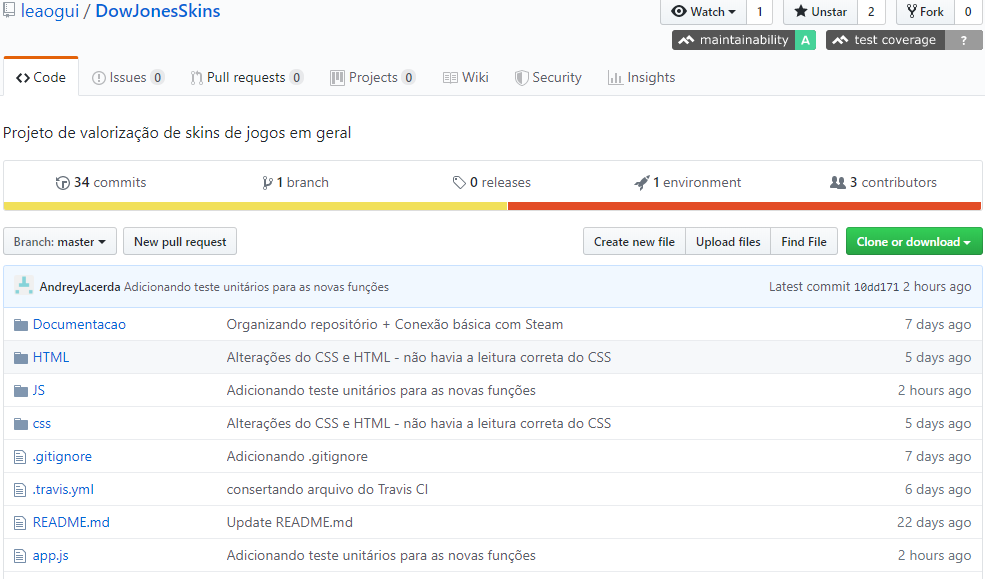
\includegraphics[scale=0.6]{Imagens/Repositorio.png}
	\caption{Repositório do Projeto no GitHub}
\end{figure}

\subsection{Instalação dos Frameworks}
Dentro da pasta raíz do projeto, o comando 'npm init' foi executado via CMD. Para isso, o Node.js foi instalado
nas máquinas dos integrantes do projeto. Este comando criou três arquivos: node\_modules, que consiste no diretório onde todos
os módulos e bibliotecas utilizadas são salvas; package.json, que consiste em um 'arquivo de configuração',
possuindo informações sobre a execução do project; package-lock.json, que consiste em um arquivo que salva
informações de todas as biliotecas e dependencias instaladas no projeto.

Com esses três arquivos criados, o Jest foi instalado, a partir do comando 'npm install jest', e o Cucumber, a partir
do comando 'npm install cucumber'. Ambos os frameworks são utilizados para testes.

Após a instalação dos dois frameworks para o node.js, os dois frameworks foram instalados para o próprio repositório do GitHub.
O primeiro foi o CodeClimate. Para isso, o dono do repositório instalou a extensão CodeClimate no navegador,
e posteriormente entrou no git do projeto. Dentro do GitHub do projeto, uma opção apareceu para adicionar
o projeto ao CodeClimate. Após clicar na opção, o repositório foi lido e adicionado ao CodeClimate, 
que agora é o plugin de avaliação de código do repositório.

Após isso, o dono do repositório instalou o Travis CI pelo próprio 'GitHub MarketPlace'.

\subsection{Criação e configuração do Heroku}
Para a criação do app no Heroku, o Heroku CLI foi instalado. Com ele instalado, o comando
'heroku create' foi executado via CMD, criando o app no Heroku. Após criar o Heroku App, o deploy do Heroku foi configurado
para que ele seja sincronizado com o 'push' para o repositório no GitHub.\\
\begin{figure}[!htb]
	\centering
	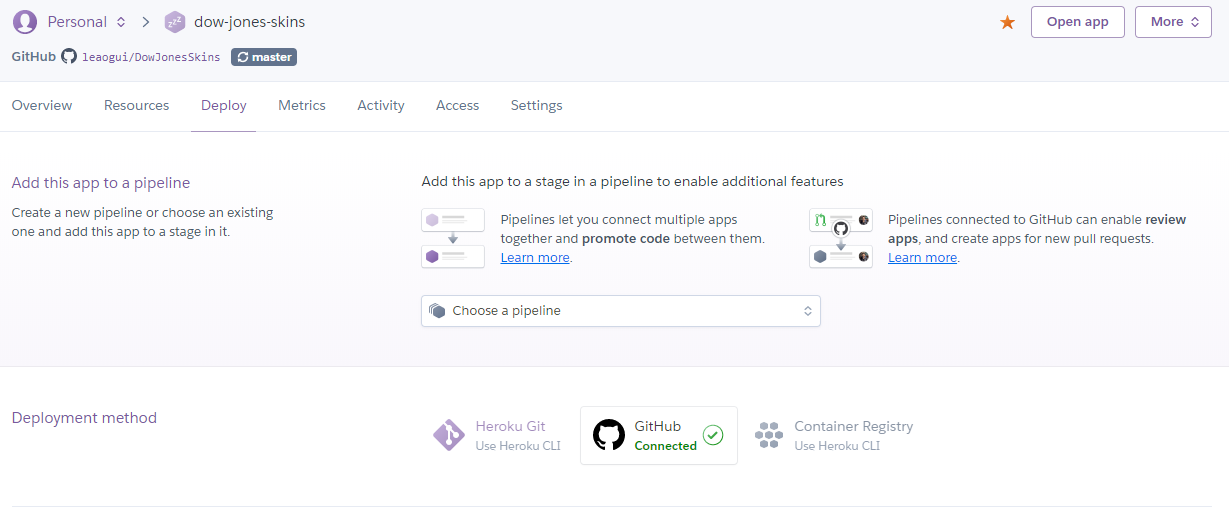
\includegraphics[scale=0.5]{Imagens/Heroku.png}
	\caption{App do Projeto no Heroku}
\end{figure}

\subsection{Home.html + app.js}
Para criar o esboço da Home do projeto, o HTML5 foi utilizado. Para estilização, o Bulma foi explorando,
que consiste num FrameWork de CSS. Cada arquivo foi separado em pastas baseadas em suas extensões. 
Diante disso, uma pasta HTMl, uma CSS e uma JS foram criadas. Na pasta CSS, o .min.css do Bulma foi salvo, para que fosse possível utilizá-lo.

Com a Home criada, o próximo passo foi o primeiro contato com o login via Steam. Para isso, a API
da Steam para Node.JS foi utilizada. No arquivos app.js, que consiste no arquivo 'main', todas as rotas foram criadas
e o framework "express" foi utilizado para instanciação do servidor web. Neste arquivo, as rotas da API Steam foram implementadas, configurando
o middleware, informando a API Key e domínio. Por conta da execução ser tanto localmente quanto no Heroku, 
vários arquivos JS com functions fororam modularizados para realizar essa troca de domínio, porta e API Key, já que tais keys mudam para cada domínio (local e Heroku). 

Para essas funções foram criadas testes unitários utilizando o Jest. Esses testes estão na subpasta 'tests' 
dentro da pasta 'JS'.\\

\begin{figure}[!htb]
	\centering
	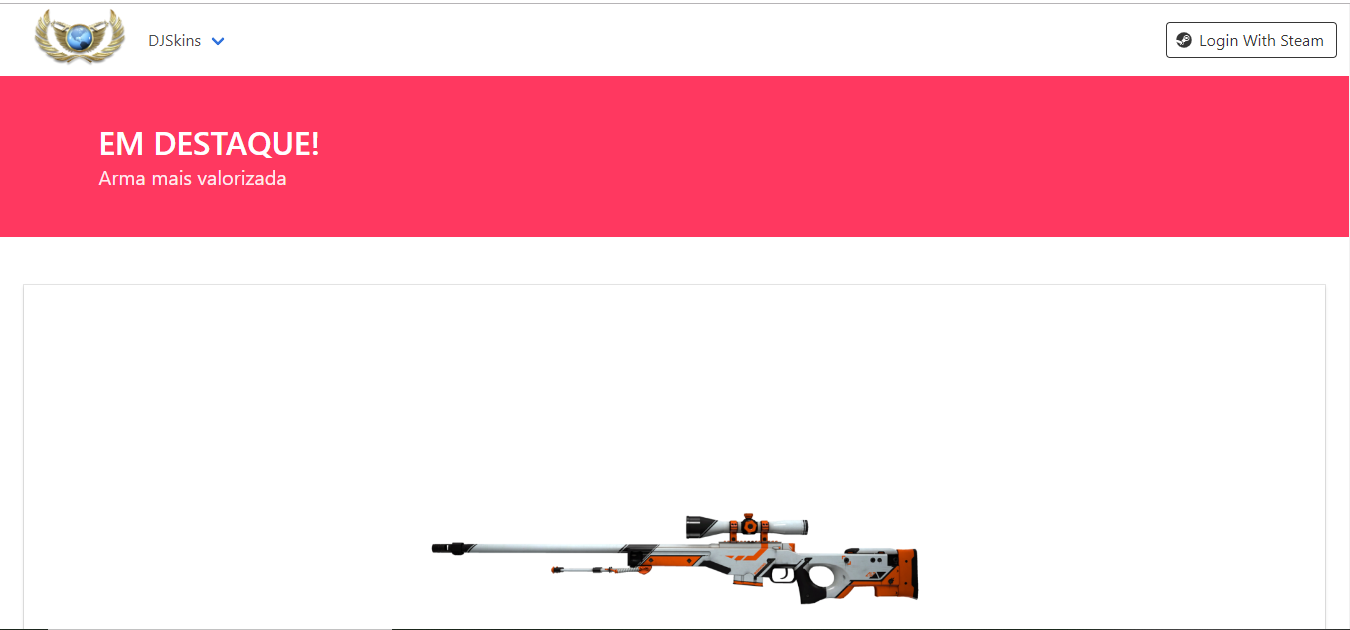
\includegraphics[scale=0.5]{Imagens/Home.png}
	\caption{Esboço da Home pronto}
\end{figure}

\subsection{Engenharia de Software}
No PivotalTracker criado pelo professor Daniel, as primeiras User Stories foram inseridas. Essas Stories consistem 
nas principais funcionalidades de usuários identificadas pelo grupo e divididas até então. Após a inserção, 
Uma pontuação foi atribuída para cada uma, a partir de um debate, onde o integrante que deu a menor nota defendia seu argumento 
junto ao integrante de deu a maior nota. O melhor argumento decide a nota.

Após isso, a prioridade e dependencias de cada User Story foi organizada, além de lançar algumas Users Stories no IceBox\\

\begin{figure}[!htb]
	\centering
	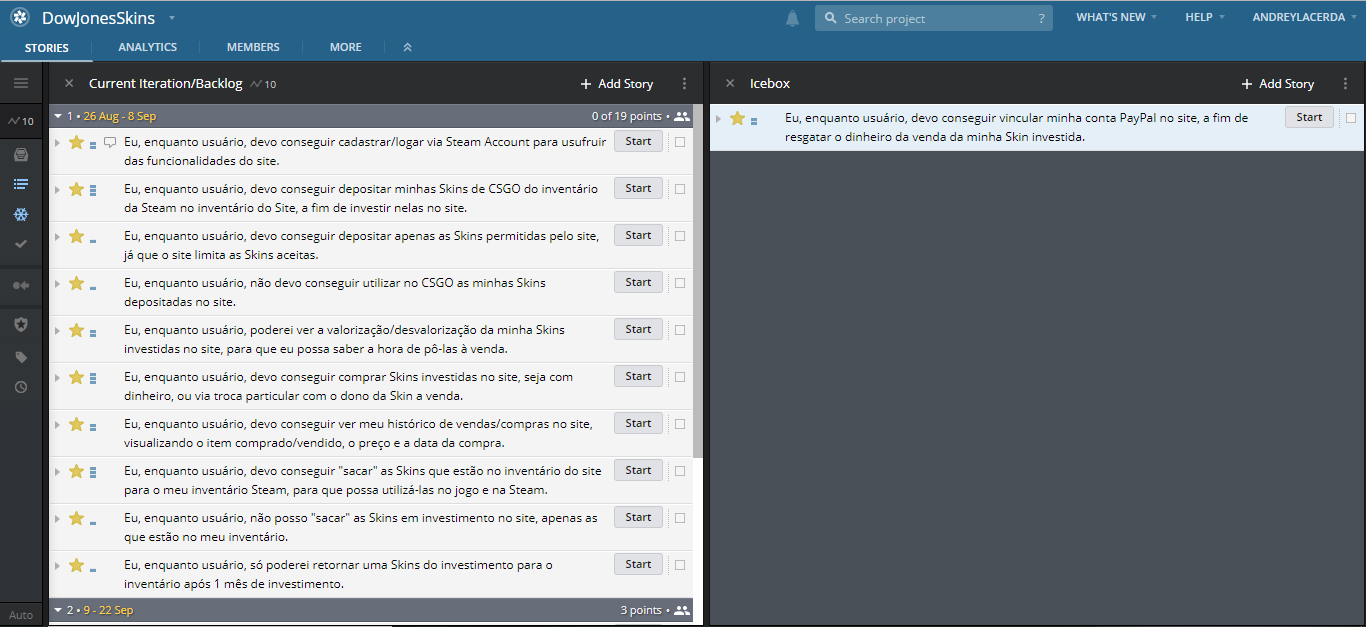
\includegraphics[scale=0.4]{Imagens/Pivotal1.png}
	\caption{PivotalTracker no 1$^{\circ}$ Sprint}
\end{figure}

\section{2$^{\circ}$ Sprint}
\subsection{Descrevendo as features com Cucumber}
Com as User Stories definidas, o passo seguinte foi esboçar todas as features utilizando o ideal do BDD 
e utilizando o Cucumber para isso. Com isso, os possíveis cenários de todas as User Stories foram descritos até então, seguindo como base o projeto exemplo mostrado pelo professor Daniel, 
mais a própria documentação do Cucumber.

Como Dito anteriormente, para isso a sintaxe do Cucumber foi utilizada, e cada feature foi separada em um arquivo diferente, 
salvas em uma pasta separada, chamada 'Features'. 
Como sintaxe, cada User Storie foi salva como Feature, com suas descrições, Backgrounds, e assim Cenários.

\subsection{Testando cadastro/login com PostgreSQL do Heroku}
Para começar o sistema de cadastro/login, o add-ons do PostGre foi adicionado ao Heroku via Heroku CLI. Para isso, 
o comando 'npm install pg' foi utilizado para instalar o Postgres do projeto. Após isso, o add-on do Postgre foi instalado no
Heroku via CMD, com comando 'heroku addons:create heroku-postgresql:hobby-dev'. Após isso, os passos 
que estão na documentação do Heroku Postgre foram seguidos, encontrados em 'https://devcenter.heroku.com/articles/heroku-postgresql'.

Após isso, as tabelas foram criadas via CMD, usando comando 'heroku psql' e adicionando todas as linhas de comando sql.
Tendo a conexão estável e as tabelas criadas, uma classe chamada 'UserCRUD' foi desenvolvida, e nela o JSON 
enviado pela Steam após conexão foi utilizado para salvar um usuário novo no banco de dados.

Nessa classe, a função signUp() recebe o JSON da Steam, conecta ao banco de dados e verifica se este usuário 
já foi cadastro. Se sim, mais nada é feito, mas caso contrário, o usuário é inserido no banco de dados.
Tendo isso feito, a primeira parte do sistema de cadastro/login foi finalizada.

\subsection{Estabelecendo Sessão}
A fim de estabelecer o sistema de login, a utilização de sessão para bloquear o acesso de usuário a 
determinadas páginas do site foi a solução mais viável. Para isso, a constante Session da biblioteca 'Express' foi utilizada.

O comando app.use() foi utilizado para usar o Session. Neste etapa, um id paraa sessão foi inserido dentro do 
parâmetro de inicialização 'secret', e false foi posto nos outros dois itens de inicialização, saveUninitialized e resave, que, 
após pesquisar, foi decidido que não fariam sentido algum.

Após isso, dentro da página '/verify' foi colocada a criação da sessão de acordo com o login do usuário na Steam. 
Com o usuário autenticado via Steam, o comando 'req.session.user' foi itilizado e o JSON fornecido pela Steam 
foi atribuído à essa constante.

Com isso, uma sessão é criada para cada usuário logado, e após isso, para bloquear o acesso à páginas sem que o user 
esteja logado, um 'IF' foi inserido em cada get do servidor (ignorando a /index e a /login). Dentro do IF, 
'!req.session.user' foi inserido, mostrando que caso não exista ression, o usuário deveria ser redirecionado para a 
tela de login da Steam, finalizando assim o ideal de sessão do site. 

\subsection{Visualizando o inventário Steam do usário}
Para obter acesso ao inventário Steam do usário logado, a biblioteca 'steam-inventory-api' foi utilizada. 
O serviço da API é inicializado quando o servidor sobe. Após isso, ao se loga na Steam, o usuário é redirecionado para o '/verify' onde, 
além de ter a sessão instanciada, os itens de seu inventário são visualizados.

Para isso, a steamId do usuário de dentro do JSON fornecido pela Steam foi recuperada e inserida como um dos diversos parâmetros da API de 
inventário. Constantes foram utilizadas para facilitar o preenchimentos dos outros parâmetros de inicialização, seguindo como base o 
exemplo de uso da API fornecido em 'https://www.npmjs.com/package/steam-inventory-api'.

Com isso, ao logar no Steam, o sistema consegue capturar todos os itens trocáveis do inventário do usário, 
além de filtrar para o jogo 'CSGO'.


\section{3$^{\circ}$ Sprint}
\subsection{Personalização via Cookie}
A fim personalizar a tela do usuário logado, cookies foram utilizados para 
exibir seu avatar e seu username. Para isso, o JSON disponibilizado pela steam logo 
após a autenticação do usuário é salvo no cookie e posteriormente resgatado por duas 
funções JavaScript encarregadas de resgatar o avatar e o username do user.

Com isso, o avatar do usuário foi printado na navbar de todas as telas, enquanto logado, enquanto seu nome 
aparece na página 'Minha Conta'.

\subsection{Template Engine Handlebars}
Conforme o projeto foi evoluindo, sua complexidade foi aparecendo. Sabendo que seria necessário o retorno 
de muita informação do banco de dados para a tela da aplicação, além de muitas regras que resultariam 
em manipulação do banco, tornou-se necessária a utilização de um Template Engine, tornando a aplicação 
inteiramente back-end. 

Diante disso, o ‘Handlebars’ foi instalado no sistema e marcado como template engine. Após isso, todos 
os HTMls desenvolvidos até então foram trocados para Handlebars, e as devidas alterações no back-end 
foram realizadas.

O HBS foi a escolha por conta de sua natureza totalmente virada para o Node.js, o qual foi utilizado 
para o back-end inteiro, e por conta de seu fácil aprendizado e resultado que solucionaria os 
problemas do projeto.

\section{4$^{\circ}$ Sprint}
\subsection{Mecânica de Depósito e Saque de Skins}
A fim de criar a mecânica de deposito e saque de skins, a API ‘steam-inventory’ foi utilizada, 
junto a algumas funções próprias.

Ao acessar o próprio inventário do DJS, a API ‘steam-inventory’ é utilizada, retornando todas as 
skins trocáveis de Counter-Strike: Global Offensive. Com essa informação, o nome de tais skins são 
printadas na tela do usuário em uma coluna a esquerda da tela, enquanto apenas as aceitadas pelo site 
são printadas na coluna do meio. Na coluna a direita, por sua vez, foi utilizada para printar as 
skins já depositadas no site pelo usuário. 

Com todas as informações na tela, botões foram adicionados. Na coluna do meio, botões que chamam 
uma função para investir a skin clicada foram adicionados, enquanto na coluna a direita, botões 
para sacar skin e investir na skin foram adicionados. A coluna a esquerda ficou apenas com nomes 
de skins.

Os botões chamam funções, que por sua vez, realizam as devias validações e manipulações no banco 
de dados, possibilitando assim o mecanismo de deposito e saque.

Devido a burocracias com a Steam, não foi possível criar uma conta para realizar as trocas reais 
de skins. Com isso, ao depositar uma skin, tal skin não some do inventário real do usuário, 
apenas é mapeado para dentro do inventário do DJS. A mesma coisa para o saque, em que a 
skin é realmente enviada para a Steam, mas sim apenas retirada do inventário do DJS, 
simulando tal troca.

\subsection{Mecânica de Investimento de Skins}
A fim de investir na skin, mecanismo core da aplicação, o botão na ‘Investir’ foi criado 
para cada skin no inventário DJS do usuário. Ao clicar no botão, uma função é invocada, 
que realiza a confirmação do investimento da skin, marcando a data do investimento.
Com a data marcada, o usuário não pode retirar o investimento até bater 31 dias, que 
consiste em outro User Story do projeto.

A fim de simular a flutuação de valores das skins do mercado, ao investir em uma skin, 
caso a skin investida é a primeira no sistema inteiro, seu valor aumenta 
15\%. Caso contrário, cai 3\%.

\section{5$^{\circ}$ Sprint}
\subsection{Mecânica de Carteira}
Após a implementação do deposito, saque e investimento de skins, a mecânica de carteira foi 
desenvolvida para possibilitar a compra de skins. Para isso, foi criado uma sessão ‘Carteira’, e 
uma coluna ‘saldo’ na tabela ‘usuario’ do Postgresql. 

Ao clicar em ‘Depositar’ na sessão de ‘Carteira’, automaticamente R\$15 creditados em seu ‘saldo’, 
realizando um UPDATE no banco de dados. Ao informar uma quantia a sacar e clicar em ‘Retirar’, tal 
quantia é validada com o saldo. Se o saldo for maior ou igual a quantia, tal valor é debitado do 
saldo, realizando outro UPDATE no banco de dados.

\subsection{Mecânica de Compra de Skins e Histórico de Vendas}
Para o mecanismo de compra, foi criado a sessão ‘DayTrade’, em que o usuário 
acessará para ver todas as skins investidas no site e seu determinado preço, além 
de ver seus próprios investimentos, possibilitando o cancelamento de algum deles, 
caso tenham mais de 31 dias.

Com isso, ao encontrar um skin que deseja, o usuário clica em ‘Comprar’, e uma função é 
chamada para validar a compra. Se a compra for válida, o usuário comprador recebe a skin 
do usuário “vendedor” que está a mais tempo com o investimento aberto. Com isso, do saldo do 
comprador é debitado o valor da skin, enquanto do saldo do vendedor é creditado tal valor. 

Além disso, um histórico de vendas é criado, marcando assim o nome do vendedor/comprador, as 
informações da skin comprada e a data da compra. Tal histórico também pode ser visto na tela 
‘DayTrade’.

\subsection{Testes}
Após todos os desenvolvimentos serem concluídos e testados pela equipe, o desenvolvimento de 
teste automatizados foram realizados. Para isso, o framework de testes Jest foi utilizado para 
o testes unitários e de integração, enquanto o Puppeteer e o Cucumber foram utilizados para os 
testes End-To-End. 

Ao total, dezesseis testes foram implementados, testando as funcionalidades principais do sistema, 
evitando qualquer má manipulação de banco de dados e interferência no mecanismo de valorização de
skins do site.

Além desses testes, uma ferramenta de análise estática foi utilizada no projeto. Tal ferramenta 
foi o ‘jshint’, e serviu como “cleaner” de “code smells”. A análise estática de 100\% ao final 
das refatorações requisitadas pela ferramenta.

%\section{Tipo de Pesquisa}
%\lipsum[3-5]

%\section{Plano Amostral (se Pesquisa Quantitativa)}
%\lipsum[3-5]

%\section{Instrumento de Pesquisa e Escalas Utilizadas (Escalas se Pesquisa Quantitativa)}
%\lipsum[3-5]

%\section{Coleta de Dados}
%\lipsum[3-5]

%\section{Análise de Dados}
%\lipsum[3-5]


%---------------------------------------------------------------------------------------


%---------------------------------------------------------------------------------------
%\chapter{Considerações finais}
%\lipsum[3]

%\section{Resposta à Questão de Pesquisa}
%\lipsum[3-5]

%\section{Objetivos Propostos}
%\lipsum[3-5]

%\section{Contribuições Academicas e Gerenciais}
%\lipsum[3-5]

%\section{Limitações da Pesquisa e Contribuições para Estudo}
%\lipsum[3-5]





% exemplos de escrita LaTeX
%\chapter{Exemplos \LaTeX}


% exemplo de como inserir uma referencia adicional no sumario (normalmente não utilizado em um trabalho academico)
\addcontentsline{toc}{chapter}{Exemplos que devem ser lidos :-)}

Esse capítulo tem exemplos de escrita utilizando o \LaTeX  utilizando \abnTeX, é muito simples escrever em \textbf{negrito}, \emph{italico}, ....


Existem diversos tutoriais para uso de \LaTeX, se você está utilizando esse modelo não precisará se preocupar com muitos dos detalhes técnicos do \LaTeX \space e cuidar somente do seu texto.

Escolha seu editor : \url{https://en.wikipedia.org/wiki/Comparison\_of\_TeX\_editors}


\section{Normas ABNT}

Leia os documentos do \abnTeX e do IFSP :
\begin{itemize}
    \item \url{http://www.abntex.net.br/}
    
    \item \acs{faq} : \url{https://github.com/abntex/abntex2/wiki/FAQ}
    
    \item \url{http://mirror.unl.edu/ctan/macros/latex/contrib/abntex2/doc/abntex2.pdf}
    
    \item \url{https://spo.ifsp.edu.br/biblioteca?id=184}
\end{itemize}

No IFSP você pode acessar todas as normas ABNT sem custo, as informações estão disponíveis no endereço \url{http://www.ifsp.edu.br/index.php/outras-noticias/52-reitoria/2329-alunos-e-servidores-do-ifsp-podem-acessar-abnt-via-web.html}



\section{Detalhes textuais}

O documento é dividido em capítulos, e cada capítulo dividido em seções utilizando o \abnTeX \space você pode dividir seus documentos nos níveis a seguir:

\begin{itemize}
\item chapter (1);
\item section (1.1);
\item subsection (1.1.1);
\item subsubsection (1.1.1.1);
\item subsubsubsection (1.1.1.1.1).
\end{itemize}

Tenha em mente que normalmente se utiliza no máximo o nível \emph{subsection}.
Ao definir as divisões do seu trabalho utilizando as diretivas do \LaTeX, elas são automaticamente inseridas no sumário do documento.


\subsection{Caracteres Reservados}



Alguns caracteres são reservados no \LaTeX \space e por isso para utilizar esses caracteres é necessario utilizar uma forma diferenciada de escrita. É possivel utilizar a macro \emph{symbol} com o codigo ascii do caracter desejado.
\begin{itemize}
\item barra invertida : \textbackslash   \symbol{92}    $\backslash$;
\item til  :  \symbol{126} ;
\item cifrão : \$;
\item sublinhado, \emph{underscore}, \emph{underline} : \_;
\item chaves : \} \{.
\end{itemize}


\chapter*[Referências]{Referências}
\addcontentsline{toc}{chapter}{Referências}
	\noindent
	DOCUMENTAÇÃO HEROKU POSTGRESQL. HEROKU.
	Disponível em: \textless
	https://devcenter.heroku.com/articles/heroku-postgresql\textgreater. Acesso em: 04 Out. 2019. \\
	
	\noindent
	DOCUMENTAÇÃO STEAM-INVENTORY-API.
	Disponível em: \textless
	'https://www.npmjs.com/package/steam-inventory-api'\textgreater. Acesso em: 02 Out. 2019. \\
    
    \noindent
    ITENS ‘COSMÉTICOS’ MOVIMENTAM CULTURA E ECONOMIA DOS JOGOS. E-Arena. Disponível em: \textless https://e-arena.com.br/itens-cosmeticos-movimentam-cultura-e-economia-dos-jogos/\textgreater. Acesso em: 14 Out. 2019. \\
    
    \noindent
    MERCADO DE SKINS DE CS:GO PODE MOVIMENTAR ATÉ 10 BILHÕES DE DÓLARES POR ANO. The Enemy. Disponível em:\textless https://www.theenemy.com.br/esports/csgo-mercado-skins-10-bilhoes-valores-precos\textgreater. Acesso em: 14 Out. 2019. \\
    
    \noindent
    NEWZOO ARTICLES. NewZoo. Disponível em: \textless https://newzoo.com/insights/articles/\textgreater. Acesso em: 15 Out. 2019. \\
    
    \noindent
    PUC PR. Mercado De Jogos Digitais Cresce No Brasil E No Mundo. G1 Globo, 08/10/2018. Disponível em: \textless https://g1.globo.com/pr/parana/especial-publicitario/puc-pr/profissionais-do-amanha/noticia/2018/10/08/mercado-de-jogos-digitais-cresce-no-brasil-e-no-mundo.ghtml\textgreater. Acesso em: 15 Out. 2019. \\
    
    \noindent
    SETOR DE GAMES CRESCE ACIMA DA MÉDIA NO PAÍS, MAS É O 13º DO MUNDO. O Tempo. Disponível em: \textless https://www.otempo.com.br/economia/subscription-required-7.5927739?aId=1.2224441\textgreater. Acesso em: 15 Out. 2019. \\
    

%Existem diversas formas de citação observe os exemplos :

%\begin{itemize}
%    \item \cite{UML:JACOBSON} | \cite{POWELL:2006} \\ 
%        \cite{SCRUMGUIDE:2013} | \cite{urani1994} |\\
%        \cite{ETAL5} | \cite{ETAL4}
%
%    \item \citeonline{UML:JACOBSON} | \citeonline{POWELL:2006} \\
%        \citeonline{SCRUMGUIDE:2013} | \citeonline{urani1994} | \\
%        \citeonline{ETAL5} | \citeonline{ETAL4}
%
 %   \item \citeauthoronline{UML:JACOBSON}| \citeauthoronline{POWELL:2006} \\
 %       \citeauthoronline{SCRUMGUIDE:2013} | \citeauthoronline{urani1994} | \\
 %       \citeauthoronline{ETAL5} | \citeauthoronline{ETAL4}
%
 %   \item \citeauthor{UML:JACOBSON}| \citeauthor{POWELL:2006} \\
 %       \citeauthor{SCRUMGUIDE:2013}| \citeauthor{urani1994} | \\
 %       \citeauthor{ETAL5} | \citeauthor{ETAL4}
 %       
 %   \item \url{http://mirrors.ibiblio.org/CTAN/macros/latex/contrib/abntex2/doc/abntex2cite-alf.pdf}
%\end{itemize}
%
%Os dados devem ser definidos corretamente nos arquivos \textquote{.BIB} para a correta formatação no texto e na lista de referências.
%
%Palavras que devem ser apresentadas no glossário devem ser citadas especificamente no texto utilizando os comandos de glossário como : \gls{tag}
%
%
%Abreviaturas podem ser referenciadas diretamente 
%na versão reduzida \textquote{\acs{ifsp}} \space  
%ou longa \textquote{\acl{ifsp}}
%
%\begin{itemize}
%    \item Autor com diversas publicações no mesmo ano : \url{https://github.com/abntex/biblatex-abnt/issues/20}
%\end{itemize}


\subsection{Listas}

Em uma lista de itens cada item deve ser terminado por ponto e virgula, exceto o ultimo item que deve ter um ponto final.

\begin{itemize}
\item item 1;
\item item 2;
\item item ..;
\item item final.
\end{itemize}

\subsection{Elementos não textuais}

Elementos não textuais são aqueles que auxiliam o entendimento, não podem ficar "jogados" no texto, devem ser citados, cada elemento deve ser identificado por um \emph{label} único que permite a sua referencia, no texto utilizando \emph{ref} ou \emph{autoref}, esses elementos quando definidos corretamente também são inseridos nas listas presentes antes do sumário.

Lembre que o \LaTeX \  vai posicionar os elementos  da melhor maneira possível dentro do documento, sempre faça as referencias utilizando os comandos específicos, nunca utiliza "acima", "baixo", "a seguir", etc...

O posicionamento desses elementos é feito pelas rotinas do pacote float, leia a documentação em  \url{http://linorg.usp.br/CTAN/macros/latex/contrib/float/float.pdf}. A opção H deverá ser utilizada somente como ultima alternativa de posicionamento.





\subsection{Tabelas e Quadros}
A ‘norma’ 14724 \cite[3.32]{NBR14724:2011} define a Tabela como sendo uma "forma não discursiva de apresentar informações das quais o dado numérico se destaca como informação central" 

Quadros e tabelas são informações tabulares, mas Tabelas tem como objetivo apresentar números.

Uso de tabelas no \LaTeX : \url{https://en.wikibooks.org/wiki/LaTeX/Tables}

Antes de utilizar longtable procure reorganizar o seu layout ou quebrar manualmente em multilplos quadros / tabelas.



\index{quadros}O \autoref{quadro-exemplo} é um exemplo de dados tabulares gerados em 
\LaTeX.

\begin{quadro}[htb]
\centering
\ABNTEXfontereduzida
\caption[Níveis de investigação]{Níveis de investigação.}
\label{quadro-exemplo}
\begin{tabular}{|p{2.6cm}|p{6.0cm}|p{2.25cm}|p{3.40cm}|}
  \hline
   \textbf{Nível de Investigação} & \textbf{Insumos}  & \textbf{Sistemas de Investigação}  & \textbf{Produtos}  \\
    \hline
    Meta-nível & Filosofia\index{filosofia} da Ciência  & Epistemologia &
    Paradigma  \\
    \hline
    Nível do objeto & Paradigmas do metanível e evidências do nível inferior &
    Ciência  & Teorias e modelos \\
    \hline
    Nível inferior & Modelos e métodos do nível do objeto e problemas do nível inferior & Prática & Solução de problemas  \\
   \hline
\end{tabular}
\legend{Fonte: Próprio Autor}
\end{quadro}



\index{tabelas}Já a \autoref{tab-exemplo} foi criada conforme o padrão do \ac{ibge}
requerido pelas normas da \ac{abnt} para documentos técnicos e acadêmicos. Observe que não existem bordas laterais em uma Tabela e os números devem ser alinhados a direita.

\begin{table}[htb]
\centering
\caption{Um Exemplo de tabela}
\label{tab-exemplo}
\begin{tabular}{p{2.6cm}|r|r|r}
    \hline
   \textbf{Item} & \textbf{Janeiro}  & \textbf{Fevereiro}  & \textbf{Março}  \\
    \hline
    Classes & 2  & 10 & 20  \\
    \hline
    Linhas & 100  & 250 & 543 \\
    \hline
\end{tabular}
\fonte{Dados do Projeto}
\end{table}

\def\equationautorefname~#1\null{%
  Equação~(#1)\null
}


Para facilitar a criação de tabelas e quadros existem algumas ferramentas como o Tables Generator \url{http://www.tablesgenerator.com/latex_tables} que permite a criação de forma visual gerando o código \LaTeX\ correspondente.


\index{equação}\index{Pitagoras}A \autoref{eq-pythagoras} mostra que também é possível escrever equações diretamente em \LaTeX

\begin{equation}\label{eq-pythagoras}
a^2+b^2=c^2\,.
\end{equation}






% ---
\subsection{Figuras}
\label{sec_figuras}
% ---

\index{figuras}Figuras podem ser criadas diretamente em \LaTeX,
como o exemplo da \autoref{fig_circulo}, ou inseridas a partir de arquivos externos como a \autoref{fig_logo}, que é o Logotipo do \ac{ifsp}. \index{logotipo}

As figuras externas devem possuir boa qualidade e preferencialmente serem vetorizadas para se obter o melhor resultado. Procure criar suas imagens e diagramas pensando em utilizar impressão em preto-e-branco ou escala de cinza. Isto é importante, principalmente quando se pretende publicar o trabalho, uma vez que a maioria das publicações são somente em preto-e-branco. Outro benefício é o custo de impressão, normalmente menor para páginas preto-e-branco em relação a páginas coloridas.

Para diagramas em UML o PlantUML pode ser utilizado para gerar código \LaTeX como exemplo na  \autoref{diagramauml}.


Quando existem diversos detalhes utilize \ac{png} em vez de JPG \footnote{Abreviado de \ac{jpeg}}, observe a diferença no exemplo em \url{https://tex.stackexchange.com/questions/136087/selecting-best-file-extension-for-graphics-figures-pictures}.

O número da seção que contém as informações sobre figuras é \ref{sec_figuras}.


\begin{figure}[htb]
	\begin{center}
	    \setlength{\unitlength}{5cm}
		\begin{picture}(1,1)
		\put(0,0){\line(0,1){1}}
		\put(0,0){\line(1,0){1}}
		\put(0,0){\line(1,1){1}}
		\put(0,0){\line(1,2){.5}}
		\put(0,0){\line(1,3){.3333}}
		\put(0,0){\line(1,4){.25}}
		\put(0,0){\line(1,5){.2}}
		\put(0,0){\line(1,6){.1667}}
		\put(0,0){\line(2,1){1}}
		\put(0,0){\line(2,3){.6667}}
		\put(0,0){\line(2,5){.4}}
		\put(0,0){\line(3,1){1}}
		\put(0,0){\line(3,2){1}}
		\put(0,0){\line(3,4){.75}}
		\put(0,0){\line(3,5){.6}}
		\put(0,0){\line(4,1){1}}
		\put(0,0){\line(4,3){1}}
		\put(0,0){\line(4,5){.8}}
		\put(0,0){\line(5,1){1}}
		\put(0,0){\line(5,2){1}}
		\put(0,0){\line(5,3){1}}
		\put(0,0){\line(5,4){1}}
		\put(0,0){\line(5,6){.8333}}
		\put(0,0){\line(6,1){1}}
		\put(0,0){\line(6,5){1}}
		\end{picture}
	\end{center}
	\caption{\label{fig_circulo}A delimitação do espaço}
	\fonte{Os Autores}
\end{figure}


\begin{figure}[htb]
    \centering
	
\includegraphics{\ifspprefixo/logo-02.jpg}
	\caption{\label{fig_logo}Logotipo \ac{ifsp}}
	\fonte{\ac{ifsp}}
\end{figure}



% generated by Plantuml 7997beta
\definecolor{plantucolor0000}{RGB}{254,254,206}
\definecolor{plantucolor0001}{RGB}{168,0,54}
\definecolor{plantucolor0002}{RGB}{173,209,178}
\definecolor{plantucolor0003}{RGB}{0,0,0}
\definecolor{plantucolor0004}{RGB}{0,0,255}

\begin{figure}[htb]
    \centering
\begin{tikzpicture}[yscale=-1]
\draw[color=plantucolor0001,fill=plantucolor0000,line width=1.5pt] (131pt,29pt) rectangle (223pt,90.8359pt);
\draw[color=plantucolor0001,fill=plantucolor0002,line width=1.0pt] (146pt,45pt) ellipse (11pt and 11pt);
\draw[color=black,fill=black] (148.7656pt,40.875pt) ..controls (148.9219pt,40.6563pt) .. (149.1094pt,40.5469pt) ..controls (149.2969pt,40.4375pt) .. (149.5156pt,40.4375pt) ..controls (149.8906pt,40.4375pt) .. (150.125pt,40.6953pt) ..controls (150.3594pt,40.9531pt) .. (150.3594pt,41.5625pt) -- (150.3594pt,43.0156pt) ..controls (150.3594pt,43.625pt) .. (150.125pt,43.8906pt) ..controls (149.8906pt,44.1563pt) .. (149.5156pt,44.1563pt) ..controls (149.1719pt,44.1563pt) .. (148.9688pt,43.9531pt) ..controls (148.7656pt,43.7656pt) .. (148.6563pt,43.25pt) ..controls (148.6094pt,42.8906pt) .. (148.4219pt,42.7031pt) ..controls (148.0938pt,42.3281pt) .. (147.4844pt,42.1094pt) ..controls (146.875pt,41.8906pt) .. (146.25pt,41.8906pt) ..controls (145.4844pt,41.8906pt) .. (144.8516pt,42.2188pt) ..controls (144.2188pt,42.5469pt) .. (143.7266pt,43.2969pt) ..controls (143.2344pt,44.0469pt) .. (143.2344pt,45.0781pt) -- (143.2344pt,46.1719pt) ..controls (143.2344pt,47.4063pt) .. (144.125pt,48.2266pt) ..controls (145.0156pt,49.0469pt) .. (146.6094pt,49.0469pt) ..controls (147.5469pt,49.0469pt) .. (148.2031pt,48.7969pt) ..controls (148.5938pt,48.6406pt) .. (149.0156pt,48.2031pt) ..controls (149.2813pt,47.9375pt) .. (149.4297pt,47.8594pt) ..controls (149.5781pt,47.7813pt) .. (149.7813pt,47.7813pt) ..controls (150.1094pt,47.7813pt) .. (150.3672pt,48.0391pt) ..controls (150.625pt,48.2969pt) .. (150.625pt,48.6406pt) ..controls (150.625pt,48.9844pt) .. (150.2813pt,49.3906pt) ..controls (149.7813pt,49.9688pt) .. (148.9844pt,50.2969pt) ..controls (147.9063pt,50.75pt) .. (146.6094pt,50.75pt) ..controls (145.0938pt,50.75pt) .. (143.8906pt,50.125pt) ..controls (142.9063pt,49.625pt) .. (142.2188pt,48.5547pt) ..controls (141.5313pt,47.4844pt) .. (141.5313pt,46.2031pt) -- (141.5313pt,45.0469pt) ..controls (141.5313pt,43.7188pt) .. (142.1484pt,42.5703pt) ..controls (142.7656pt,41.4219pt) .. (143.8594pt,40.8047pt) ..controls (144.9531pt,40.1875pt) .. (146.1875pt,40.1875pt) ..controls (146.9219pt,40.1875pt) .. (147.5703pt,40.3516pt) ..controls (148.2188pt,40.5156pt) .. (148.7656pt,40.875pt);
\node at (160pt,37.4531pt)[below right]{Subscriber};
\draw[color=plantucolor0001,line width=1.5pt] (132pt,61pt) -- (222pt,61pt);
\node at (137pt,65pt)[below right]{subscriberId};
\draw[color=plantucolor0001,line width=1.5pt] (132pt,82.8359pt) -- (222pt,82.8359pt);
\draw[color=plantucolor0001,fill=plantucolor0000,line width=1.5pt] (31pt,212pt) rectangle (137pt,273.8359pt);
\draw[color=plantucolor0001,fill=plantucolor0002,line width=1.0pt] (46pt,228pt) ellipse (11pt and 11pt);
\draw[color=black,fill=black] (48.7656pt,223.875pt) ..controls (48.9219pt,223.6563pt) .. (49.1094pt,223.5469pt) ..controls (49.2969pt,223.4375pt) .. (49.5156pt,223.4375pt) ..controls (49.8906pt,223.4375pt) .. (50.125pt,223.6953pt) ..controls (50.3594pt,223.9531pt) .. (50.3594pt,224.5625pt) -- (50.3594pt,226.0156pt) ..controls (50.3594pt,226.625pt) .. (50.125pt,226.8906pt) ..controls (49.8906pt,227.1563pt) .. (49.5156pt,227.1563pt) ..controls (49.1719pt,227.1563pt) .. (48.9688pt,226.9531pt) ..controls (48.7656pt,226.7656pt) .. (48.6563pt,226.25pt) ..controls (48.6094pt,225.8906pt) .. (48.4219pt,225.7031pt) ..controls (48.0938pt,225.3281pt) .. (47.4844pt,225.1094pt) ..controls (46.875pt,224.8906pt) .. (46.25pt,224.8906pt) ..controls (45.4844pt,224.8906pt) .. (44.8516pt,225.2188pt) ..controls (44.2188pt,225.5469pt) .. (43.7266pt,226.2969pt) ..controls (43.2344pt,227.0469pt) .. (43.2344pt,228.0781pt) -- (43.2344pt,229.1719pt) ..controls (43.2344pt,230.4063pt) .. (44.125pt,231.2266pt) ..controls (45.0156pt,232.0469pt) .. (46.6094pt,232.0469pt) ..controls (47.5469pt,232.0469pt) .. (48.2031pt,231.7969pt) ..controls (48.5938pt,231.6406pt) .. (49.0156pt,231.2031pt) ..controls (49.2813pt,230.9375pt) .. (49.4297pt,230.8594pt) ..controls (49.5781pt,230.7813pt) .. (49.7813pt,230.7813pt) ..controls (50.1094pt,230.7813pt) .. (50.3672pt,231.0391pt) ..controls (50.625pt,231.2969pt) .. (50.625pt,231.6406pt) ..controls (50.625pt,231.9844pt) .. (50.2813pt,232.3906pt) ..controls (49.7813pt,232.9688pt) .. (48.9844pt,233.2969pt) ..controls (47.9063pt,233.75pt) .. (46.6094pt,233.75pt) ..controls (45.0938pt,233.75pt) .. (43.8906pt,233.125pt) ..controls (42.9063pt,232.625pt) .. (42.2188pt,231.5547pt) ..controls (41.5313pt,230.4844pt) .. (41.5313pt,229.2031pt) -- (41.5313pt,228.0469pt) ..controls (41.5313pt,226.7188pt) .. (42.1484pt,225.5703pt) ..controls (42.7656pt,224.4219pt) .. (43.8594pt,223.8047pt) ..controls (44.9531pt,223.1875pt) .. (46.1875pt,223.1875pt) ..controls (46.9219pt,223.1875pt) .. (47.5703pt,223.3516pt) ..controls (48.2188pt,223.5156pt) .. (48.7656pt,223.875pt);
\node at (60pt,220.4531pt)[below right]{AccumUsage};
\draw[color=plantucolor0001,line width=1.5pt] (32pt,244pt) -- (136pt,244pt);
\node at (37pt,248pt)[below right]{subscriberId};
\draw[color=plantucolor0001,line width=1.5pt] (32pt,265.8359pt) -- (136pt,265.8359pt);
\draw[color=plantucolor0001,fill=plantucolor0000,line width=1.5pt] (221pt,191pt) rectangle (318pt,294.3438pt);
\draw[color=plantucolor0001,fill=plantucolor0002,line width=1.0pt] (240.05pt,207pt) ellipse (11pt and 11pt);
\draw[color=black,fill=black] (242.8156pt,202.875pt) ..controls (242.9719pt,202.6563pt) .. (243.1594pt,202.5469pt) ..controls (243.3469pt,202.4375pt) .. (243.5656pt,202.4375pt) ..controls (243.9406pt,202.4375pt) .. (244.175pt,202.6953pt) ..controls (244.4094pt,202.9531pt) .. (244.4094pt,203.5625pt) -- (244.4094pt,205.0156pt) ..controls (244.4094pt,205.625pt) .. (244.175pt,205.8906pt) ..controls (243.9406pt,206.1563pt) .. (243.5656pt,206.1563pt) ..controls (243.2219pt,206.1563pt) .. (243.0188pt,205.9531pt) ..controls (242.8156pt,205.7656pt) .. (242.7063pt,205.25pt) ..controls (242.6594pt,204.8906pt) .. (242.4719pt,204.7031pt) ..controls (242.1438pt,204.3281pt) .. (241.5344pt,204.1094pt) ..controls (240.925pt,203.8906pt) .. (240.3pt,203.8906pt) ..controls (239.5344pt,203.8906pt) .. (238.9016pt,204.2188pt) ..controls (238.2688pt,204.5469pt) .. (237.7766pt,205.2969pt) ..controls (237.2844pt,206.0469pt) .. (237.2844pt,207.0781pt) -- (237.2844pt,208.1719pt) ..controls (237.2844pt,209.4063pt) .. (238.175pt,210.2266pt) ..controls (239.0656pt,211.0469pt) .. (240.6594pt,211.0469pt) ..controls (241.5969pt,211.0469pt) .. (242.2531pt,210.7969pt) ..controls (242.6438pt,210.6406pt) .. (243.0656pt,210.2031pt) ..controls (243.3313pt,209.9375pt) .. (243.4797pt,209.8594pt) ..controls (243.6281pt,209.7813pt) .. (243.8313pt,209.7813pt) ..controls (244.1594pt,209.7813pt) .. (244.4172pt,210.0391pt) ..controls (244.675pt,210.2969pt) .. (244.675pt,210.6406pt) ..controls (244.675pt,210.9844pt) .. (244.3313pt,211.3906pt) ..controls (243.8313pt,211.9688pt) .. (243.0344pt,212.2969pt) ..controls (241.9563pt,212.75pt) .. (240.6594pt,212.75pt) ..controls (239.1438pt,212.75pt) .. (237.9406pt,212.125pt) ..controls (236.9563pt,211.625pt) .. (236.2688pt,210.5547pt) ..controls (235.5813pt,209.4844pt) .. (235.5813pt,208.2031pt) -- (235.5813pt,207.0469pt) ..controls (235.5813pt,205.7188pt) .. (236.1984pt,204.5703pt) ..controls (236.8156pt,203.4219pt) .. (237.9094pt,202.8047pt) ..controls (239.0031pt,202.1875pt) .. (240.2375pt,202.1875pt) ..controls (240.9719pt,202.1875pt) .. (241.6203pt,202.3516pt) ..controls (242.2688pt,202.5156pt) .. (242.8156pt,202.875pt);
\node at (254.95pt,199.4531pt)[below right]{IpSession};
\draw[color=plantucolor0001,line width=1.5pt] (222pt,223pt) -- (317pt,223pt);
\node at (227pt,227pt)[below right]{ipAddress};
\node at (227pt,240.8359pt)[below right]{specificData};
\node at (227pt,254.6719pt)[below right]{sapcOriginStateId};
\node at (227pt,268.5078pt)[below right]{apnId};
\draw[color=plantucolor0001,line width=1.5pt] (222pt,286.3438pt) -- (317pt,286.3438pt);
\draw[color=plantucolor0004] (191.942pt,90.081pt) ..controls (205.204pt,115.893pt) and (224.952pt,154.325pt) .. (241.265pt,186.076pt);
\draw[color=plantucolor0004,fill=plantucolor0004] (243.646pt,190.709pt) -- (243.0894pt,180.8759pt) -- (241.3604pt,186.262pt) -- (235.9742pt,184.5329pt) -- (243.646pt,190.709pt) -- cycle;
\node at (191.0584pt,98.9168pt)[below right]{1};
\node at (230.3817pt,166.6703pt)[below right]{1..*};
\draw[color=plantucolor0001] (162.058pt,90.081pt) ..controls (145.645pt,122.023pt) and (119.302pt,173.295pt) .. (101.824pt,207.31pt);
\draw[color=plantucolor0001,fill=plantucolor0001] (99.5252pt,211.784pt) -- (107.1969pt,205.6078pt) -- (101.8108pt,207.337pt) -- (100.0816pt,201.9509pt) -- (99.5252pt,211.784pt) -- cycle;
\node at (143.0082pt,98.7264pt)[below right]{1};
\node at (101.801pt,187.522pt)[below right]{0..1};
\end{tikzpicture}
\caption{\label{diagramauml}Exemplo de Diagrama UML gerado a partir do PlantUML}
	\legend{Fonte: Os Autores}
\end{figure}

A \autoref{fig_diag_virado} exemplifica como utilizar uma imagem qualquer em formato paisagem (página inteira). Obs: Utilizamos a imagem de forma a ilustrar o procedimento. Considere a legibilidade da figura quando for utilizar no trabalho final.

Para casos onde a figura referenciada está muito distante por algum motivo é possível fazer uma referencia indicando a página : \autorefwithpage{fig_diag_virado}

\begin{sidewaysfigure}[htb]
    \centering
	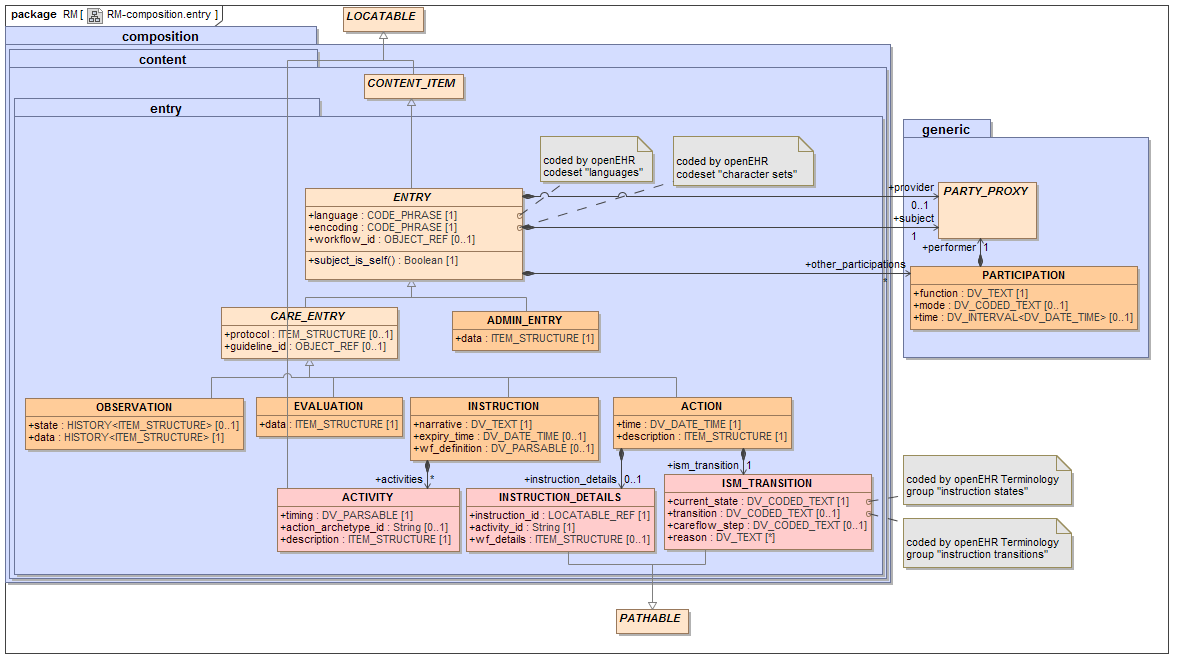
\includegraphics[width=0.9\textwidth]{exemplos/exemplo_diag_horizontal.png}
	\caption{\label{fig_diag_virado}Diagrama Virado - Exemplo}
	\fonte{\cite{openehrCompositionEntry}}
\end{sidewaysfigure}

\subsection{Organizando pendências}

Durante o desenvolvimento de um trabalho escrito é normal que alguns elementos sejam gerados posteriormente, mas é importante se organizar para não esquecer de fazer os ajustes necessários. Para isso recomendo a utilização do pacote \textbf{todonotes} que oferece diversos recursos para gerar lembretes das pendencias. O manual do \textbf{todonotes} está disponivel no \autoref{manual-todonotes}.

É possível fazer anotações de pendencias inclusive indicando as pessoas responsáveis por elas, % nao mover o todo o texto utiliza como exemplo indicando  fica assim errado
\todo[inline,author=Pessoa1]{fazer revisão das imagens do texto} e para facilitar a visualização criar imagens que funcionam como marcadores para figuras que serão incluídas posteriormente.

Cuidado ao utilizar as anotações \emph{inline} pois o texto ficara quebrado, como no paragrafo anterior.


\begin{figure}[htb]
    \centering
	\missingfigure[figwidth=10cm]{você está atrasado pois ainda não criou esta figura}
	\caption{\label{fig_todo1}Imagem que ainda não foi gerada}
	\fonte{dados do Projeto}
\end{figure}



% ---
\subsection{QR-Code}
% ---
\index{qr-code}
A utilização de códigos \ac{qr} facilita o acesso de endereços da internet a partir de dispositivos móveis com câmera.
As figuras \ref{qr-url-1} e \ref{qr-url-2} demonstram dois exemplos de endereços apresentados com essa tecnologia.


Para facilitar a utilização dos códigos \ac{qr}, deve-se tomar cuidado para não deixa-los alinhados na vertical pois dificulta a seleção a partir da câmera no dispositivo móvel.

Um exemplo para utilização de mais códigos de barra pode ser visto em : \urlmodelo.

Atenção, alguns compiladores podem ter problemas em utilizar a biblioteca \textbf{pstricks} necessária para gerar QR-Codes, no sharelatex em 2017-05 a compilação ocorre perfeitamente utilizando a opção de compilador "XeLatex", ele é mais lento que outras opções.


\begin{figure}
\begin{pspicture}(25mm,25mm)
\psbarcode{\urlmodelosimples}{eclevel=H width=1.0 height=1.0}{qrcode}
\end{pspicture}
\caption{\label{qr-url-1}QR-Code - URL Documento exemplo}
\legend{\urlmodelo}
\fonte{Os Autores}
\end{figure}



% colocando figura qrcode na direita para facilitar o uso da camera deixando cada qrcode em um alinhamento diferente
% se deixar os dois qrcodes um em cima do outro dificulta acessar o desejado
\begin{figure}
\begin{flushright}
\begin{pspicture}(25mm,25mm)
\psbarcode{https://github.com/ivanfmartinez/latexlib/tree/master/ifsp}{eclevel=H width=1.0 height=1.0}{qrcode}
\end{pspicture}
\caption{\label{qr-url-2}QR-Code - Classes IFSP GitHub}
\legend{\url{https://github.com/ivanfmartinez/latexlib/tree/master/ifsp}}
\fonte{Os Autores}
\end{flushright}

\end{figure}



\subsection{Impressão em folhas formato A3}

A página seguinte em A3 permite a impressão de diagramas grandes que não podem ser visualizados facilmente em folha padrão A4. Lembre que algumas impressoras podem ter problemas com isso, então selecione somente as páginas A4 ao imprimir e depois imprima separadamente a página A3.

A \autoref{fig_logo_A3} utiliza a mesma imagem da \autoref{fig_logo} e foi ampliada para demonstrar a essa possibilidade de impressão de grandes imagens em A3.

Observe que o código de exemplo vai gerar uma quebra de página no local onde for definida a página A3, por isso não deve ser utilizado entre textos para evitar grandes espaços em branco.

Folhas impressas em A3 ou tamanhos maiores devem ser dobradas seguindo o padrão definido pela ABNT. 


Cuidado ao utilizar folhas A3 em um documento impresso em frente e verso pois a numeração das páginas seguintes pode ser impressa de forma incorreta (posição do número na página). Uma alternativa para esta situação é manter todas páginas impressas em A3 no último apêndice.



\afterpage{%
\begin{PAGINA-A3}

\begin{figure}[p]
    \centering%
    \fcolorbox{red}{yellow}{ 
\includegraphics[height=\textheight,width=\textwidth,keepaspectratio]{\ifspprefixo/logo-02.jpg}}%
	\caption{\label{fig_logo_A3}Logotipo IFSP em página A3}
	\legend{Com borda para demonstrar os limites}
   \fonte{Autor da Figura}
\end{figure}

\end{PAGINA-A3}
}



\chapter[Diagramas]{Diagramas}
Durante o desenvolvimento do projeto, alguns diagramas foram elaborados para sincronização de pensamento da equipe e entendimento coletivo.

Como forma organização, separamos os diagramas em dois grupos, representados pelas seções a seguir.

 \section{Banco de Dados}
  Dentre os diagramas construídos, dois consistem no banco de dados, para entendimento da conexão entre as entidades do sistema, sendo um deles Diagrama de Entidade-Relacionamento, que consiste na \autoref{fig:der} e mostra o relacionamento entre as entidades do sistema, enquanto o outro consiste no Diagrama do Modelo Lógico do banco de dados da aplicação, representado na \autoref{fig:bdml}, mostrando essas relacionamentos de forma menos abstrata, já com os campos de cada tabela e seus tipos.

  \begin{figure}[!htb]
        \centering
        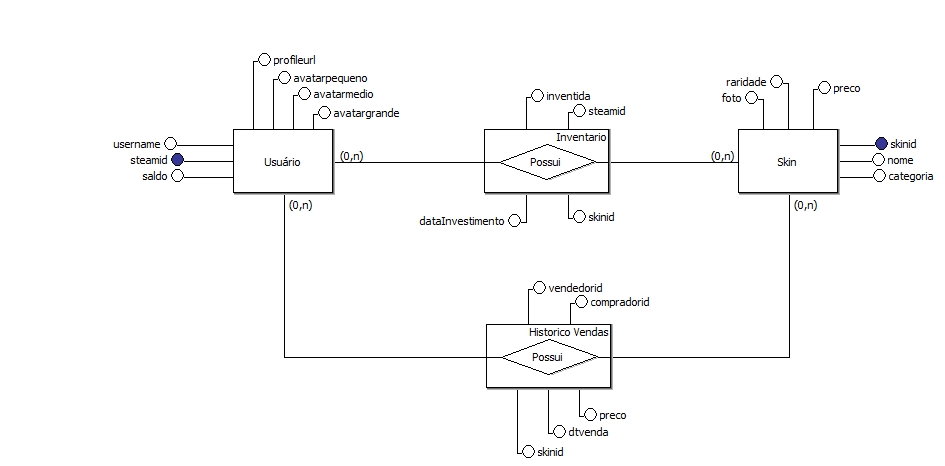
\includegraphics[scale=0.5]{Imagens/Relacionamento.png}
        \caption{Banco de Dados - Diagrama Entidade Relacionamento}
        \label{fig:der}
 \end{figure}

\begin{figure}[!htb]
	\centering
	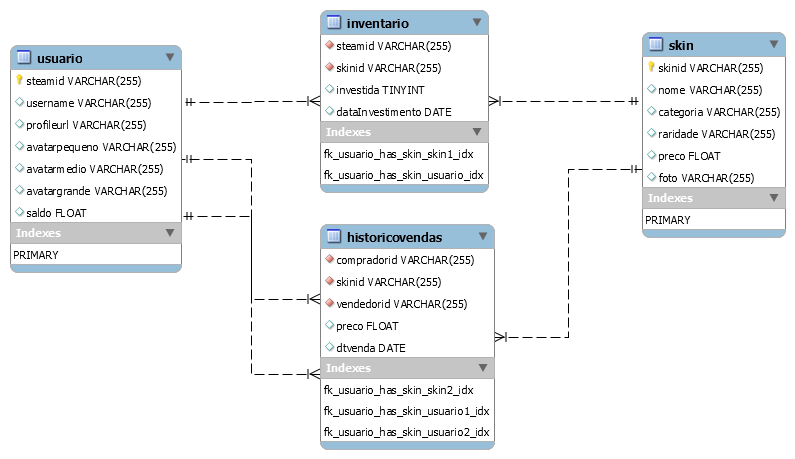
\includegraphics[scale=0.6]{Imagens/Logico.png}
	\caption{Banco de Dados - Modelo Lógico}
	\label{fig:bdml}
\end{figure}
\clearpage

\section{Diagramas de Atividade}
Além desses dois diagramas apresentados acima, três Diagramas de Atividade foram construídos para auxiliar no alinhamento de ideias do grupo e entendimento das funcionalidades. 

O diagrama representado na \autoref{fig:dami} consiste no funcionamento do mecanismo de inventário do projeto, enquanto a \autoref{fig:damdt} representa o funcionamento da mecânica de Day Trade e a \autoref{fig:damc} representa o sistema de carteira da aplicação.

	\begin{figure}[!htb]
		\centering
		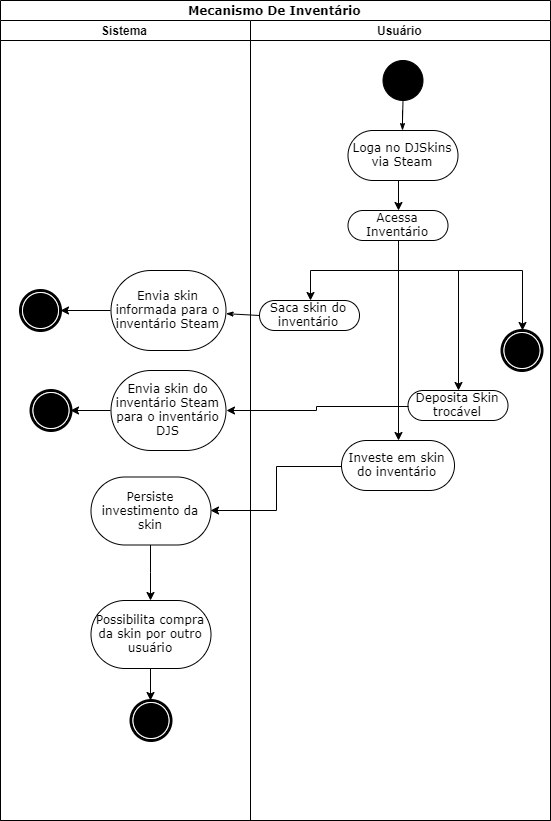
\includegraphics[scale=0.6]{Imagens/mec-inventario.png}
		\caption{Diagrama de Atividades - Mecanismo de Inventário}
		\label{fig:dami}
	\end{figure}
	
	\begin{figure}[!htb]
		\centering
		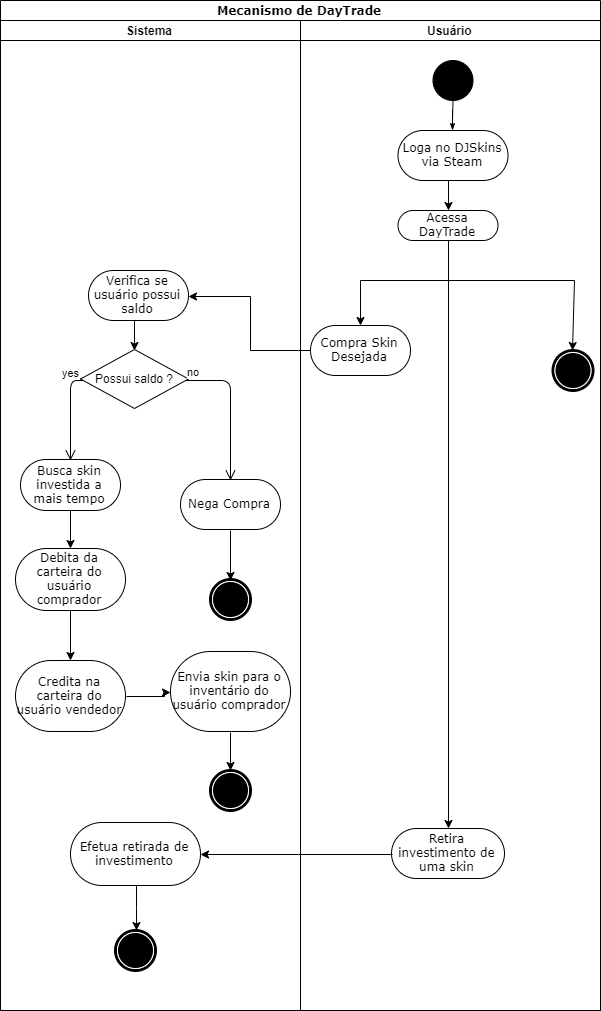
\includegraphics[scale=0.6]{Imagens/mec-daytrade.png}
		\caption{Diagrama de Atividades - Mecanismo de Day Trade}
		\label{fig:damdt}
	\end{figure}
	
	\begin{figure}[!htb]
		\centering
		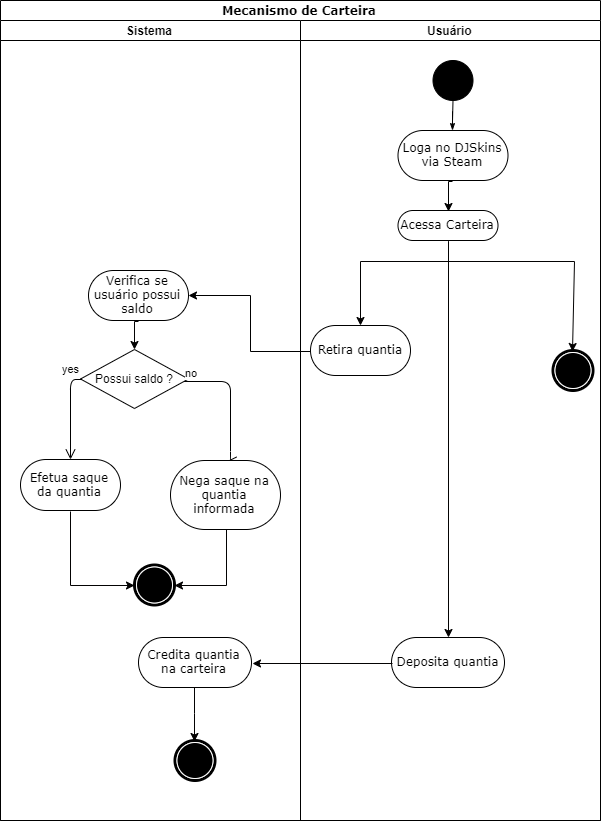
\includegraphics[scale=0.6]{Imagens/mec-carteira.png}
		\caption{Diagrama de Atividades - Mecanismo de Carteira}
		\label{fig:damc}
	\end{figure}

% ---
% Conclusão (outro exemplo de capítulo sem numeração e presente no sumário)
% ---
\chapter*[Conclusão]{Conclusão}
\addcontentsline{toc}{chapter}{Conclusão}
Em suma, o projeto construído consiste em uma aplicação web para vendas de skins do jogo 
Counter-Strike: Global Offensive.

Node.js foi utilizado para o desenvolvimento back-end,
enquanto o HTML5 foi utilizado para o front-end. Como template-engine, o handlebars foi 
utilizado, tornando a aplicação server-side.

Como metodologia de engenharia de software, os métodos ágeis foram aplicados, e o 
desenvolvimento do sistema foi feito em cima de Users Stories separadas por sprints, 
similarmente a metodologia XP.  

Para a implementação do projeto, duas APIs da Steam foram utilizadas, sendo uma para 
autenticação, e outra para resgate de inventário. O GitHub foi utilizado para como 
gerenciador de versão, enquanto o Heroku foi utilizado como ferramenta de deploy.

Além disso, foi utilizado o PostgreSQL do Heroku como banco de dados da aplicação, salvando 
assim as skin, as contas dos usuários, seus inventários e seus históricos de venda.

Como testes, testes unitários e de integração foram implementados em grande quantidade, 
enquanto um único teste end-to-end automatizado foi desenvolvido. A ferramenta de análise 
estática ‘jshint’ foi utilizada para neutralização de code smells.

Ao final de todo o desenvolvimento, a aplicação construída foi um sucesso, abraçando 
mecânicas de depósito, retirada, compra, valorização e investimento de skins, além de ter um 
mecanismo de carteira. Todos esses mecanismos feitos de forma simulada, não realizando a 
real troca ou compra de skins, assim como deposito e saque de dinheiro da carteira.

% ---


% ----------------------------------------------------------
% Finaliza a parte no bookmark do PDF
% para que se inicie o bookmark na raiz
% e adiciona espaço de parte no Sumário
% ----------------------------------------------------------
\phantompart

% ----------------------------------------------------------
% ELEMENTOS PÓS-TEXTUAIS
% ----------------------------------------------------------
\postextual
% ----------------------------------------------------------

% ----------------------------------------------------------
% Referências bibliográficas
% ----------------------------------------------------------

\chapter*[Referências]{Referências}
\addcontentsline{toc}{chapter}{Referências}
	\noindent
	DOCUMENTAÇÃO HEROKU POSTGRESQL. HEROKU.
	Disponível em: \textless
	https://devcenter.heroku.com/articles/heroku-postgresql\textgreater. Acesso em: 04 Out. 2019. \\
	
	\noindent
	DOCUMENTAÇÃO STEAM-INVENTORY-API.
	Disponível em: \textless
	'https://www.npmjs.com/package/steam-inventory-api'\textgreater. Acesso em: 02 Out. 2019. \\
    
    \noindent
    ITENS ‘COSMÉTICOS’ MOVIMENTAM CULTURA E ECONOMIA DOS JOGOS. E-Arena. Disponível em: \textless https://e-arena.com.br/itens-cosmeticos-movimentam-cultura-e-economia-dos-jogos/\textgreater. Acesso em: 14 Out. 2019. \\
    
    \noindent
    MERCADO DE SKINS DE CS:GO PODE MOVIMENTAR ATÉ 10 BILHÕES DE DÓLARES POR ANO. The Enemy. Disponível em:\textless https://www.theenemy.com.br/esports/csgo-mercado-skins-10-bilhoes-valores-precos\textgreater. Acesso em: 14 Out. 2019. \\
    
    \noindent
    NEWZOO ARTICLES. NewZoo. Disponível em: \textless https://newzoo.com/insights/articles/\textgreater. Acesso em: 15 Out. 2019. \\
    
    \noindent
    PUC PR. Mercado De Jogos Digitais Cresce No Brasil E No Mundo. G1 Globo, 08/10/2018. Disponível em: \textless https://g1.globo.com/pr/parana/especial-publicitario/puc-pr/profissionais-do-amanha/noticia/2018/10/08/mercado-de-jogos-digitais-cresce-no-brasil-e-no-mundo.ghtml\textgreater. Acesso em: 15 Out. 2019. \\
    
    \noindent
    SETOR DE GAMES CRESCE ACIMA DA MÉDIA NO PAÍS, MAS É O 13º DO MUNDO. O Tempo. Disponível em: \textless https://www.otempo.com.br/economia/subscription-required-7.5927739?aId=1.2224441\textgreater. Acesso em: 15 Out. 2019. \\
    

%Existem diversas formas de citação observe os exemplos :

%\begin{itemize}
%    \item \cite{UML:JACOBSON} | \cite{POWELL:2006} \\ 
%        \cite{SCRUMGUIDE:2013} | \cite{urani1994} |\\
%        \cite{ETAL5} | \cite{ETAL4}
%
%    \item \citeonline{UML:JACOBSON} | \citeonline{POWELL:2006} \\
%        \citeonline{SCRUMGUIDE:2013} | \citeonline{urani1994} | \\
%        \citeonline{ETAL5} | \citeonline{ETAL4}
%
 %   \item \citeauthoronline{UML:JACOBSON}| \citeauthoronline{POWELL:2006} \\
 %       \citeauthoronline{SCRUMGUIDE:2013} | \citeauthoronline{urani1994} | \\
 %       \citeauthoronline{ETAL5} | \citeauthoronline{ETAL4}
%
 %   \item \citeauthor{UML:JACOBSON}| \citeauthor{POWELL:2006} \\
 %       \citeauthor{SCRUMGUIDE:2013}| \citeauthor{urani1994} | \\
 %       \citeauthor{ETAL5} | \citeauthor{ETAL4}
 %       
 %   \item \url{http://mirrors.ibiblio.org/CTAN/macros/latex/contrib/abntex2/doc/abntex2cite-alf.pdf}
%\end{itemize}
%
%Os dados devem ser definidos corretamente nos arquivos \textquote{.BIB} para a correta formatação no texto e na lista de referências.
%
%Palavras que devem ser apresentadas no glossário devem ser citadas especificamente no texto utilizando os comandos de glossário como : \gls{tag}
%
%
%Abreviaturas podem ser referenciadas diretamente 
%na versão reduzida \textquote{\acs{ifsp}} \space  
%ou longa \textquote{\acl{ifsp}}
%
%\begin{itemize}
%    \item Autor com diversas publicações no mesmo ano : \url{https://github.com/abntex/biblatex-abnt/issues/20}
%\end{itemize}

%% ----------------------------------------------------------
% Glossário
% ----------------------------------------------------------
%
%
\ifdef{\printnoidxglossary}{
    \addcontentsline{toc}{chapter}{GLOSSÁRIO}
    \printnoidxglossary[style=glossario]
    %\printglossaries
}{}

%% ----------------------------------------------------------
% Apêndices
% Documentos gerados pelo próprio autor
% ----------------------------------------------------------

% ---
% Inicia os apêndices
% ---
\begin{apendicesenv}

% Imprime uma página indicando o início dos apêndices
\partapendices

% ----------------------------------------------------------
\chapter{Quisque libero justo}
% ----------------------------------------------------------

\lipsum[1-2]

% ----------------------------------------------------------
\chapter{Nullam elementum urna vel imperdiet sodales elit ipsum pharetra ligula
ac pretium ante justo a nulla curabitur tristique arcu eu metus}
% ----------------------------------------------------------
\lipsum[3-5]

\end{apendicesenv}
% ---

%% ----------------------------------------------------------
% Anexos
% Documentos gerados por outros autores
% ----------------------------------------------------------

% ---
% Inicia os anexos
% ---
\begin{anexosenv}

% Imprime uma página indicando o início dos anexos
\partanexos

% ---
\chapter{Manual todonotes(parcial)}
\label{manual-todonotes}
% ---
\index{pdf}
% se pages = "-"  fica com arquivo completo
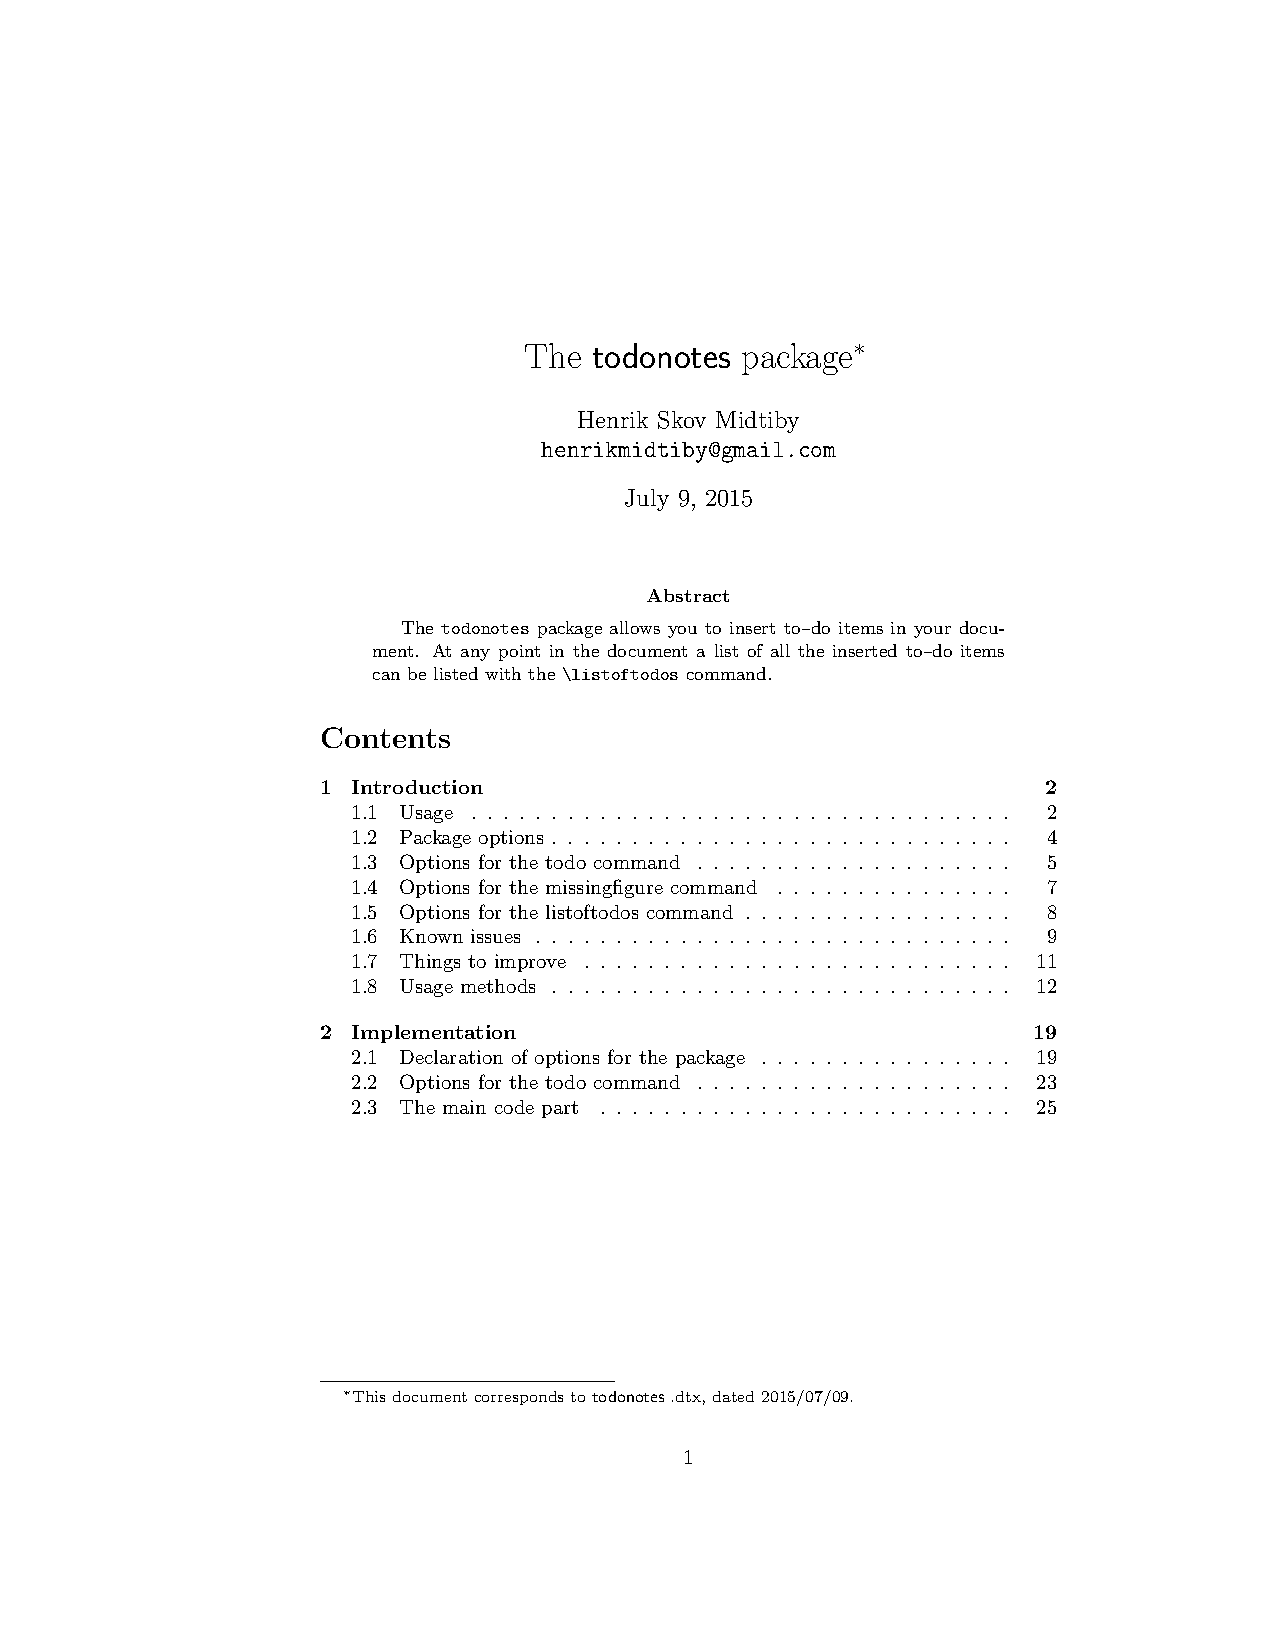
\includepdf[pages=1-3,scale=0.8,frame=true,pagecommand={}]{anexos/todonotes.pdf}

% ---
% Para incluir sem gerar a quebra de página inicial no anexo
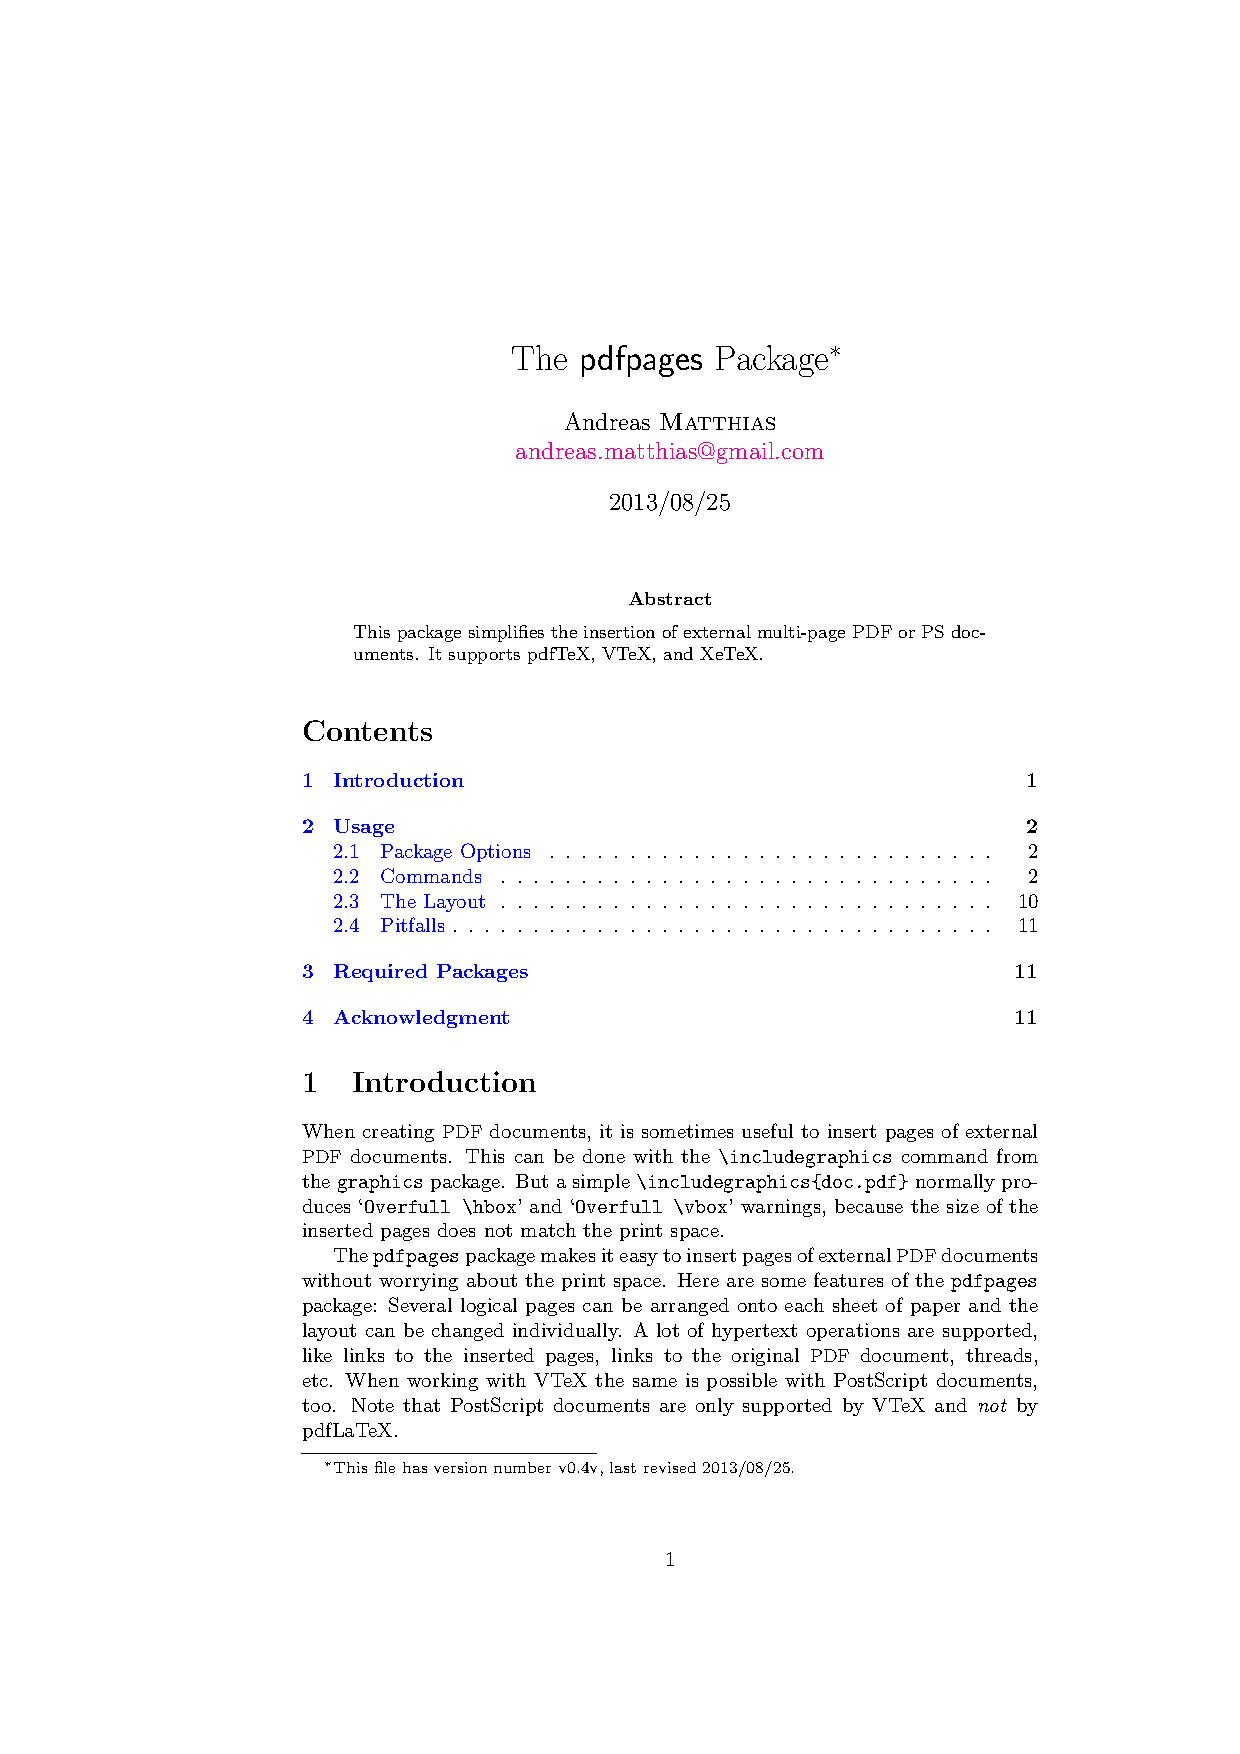
\includepdf[pages=1,scale=0.7,frame=true,pagecommand=\chapter{Manual pdfpages(parcial)}\label{manual-pdf}]{anexos/pdfpages.pdf}
\includepdf[pages=2-3,scale=0.8,frame=true,pagecommand={}]{anexos/pdfpages.pdf}

% ---
\chapter{Manual acronym(parcial)}
\index{pdf}
% somente algumas páginas para exemplo
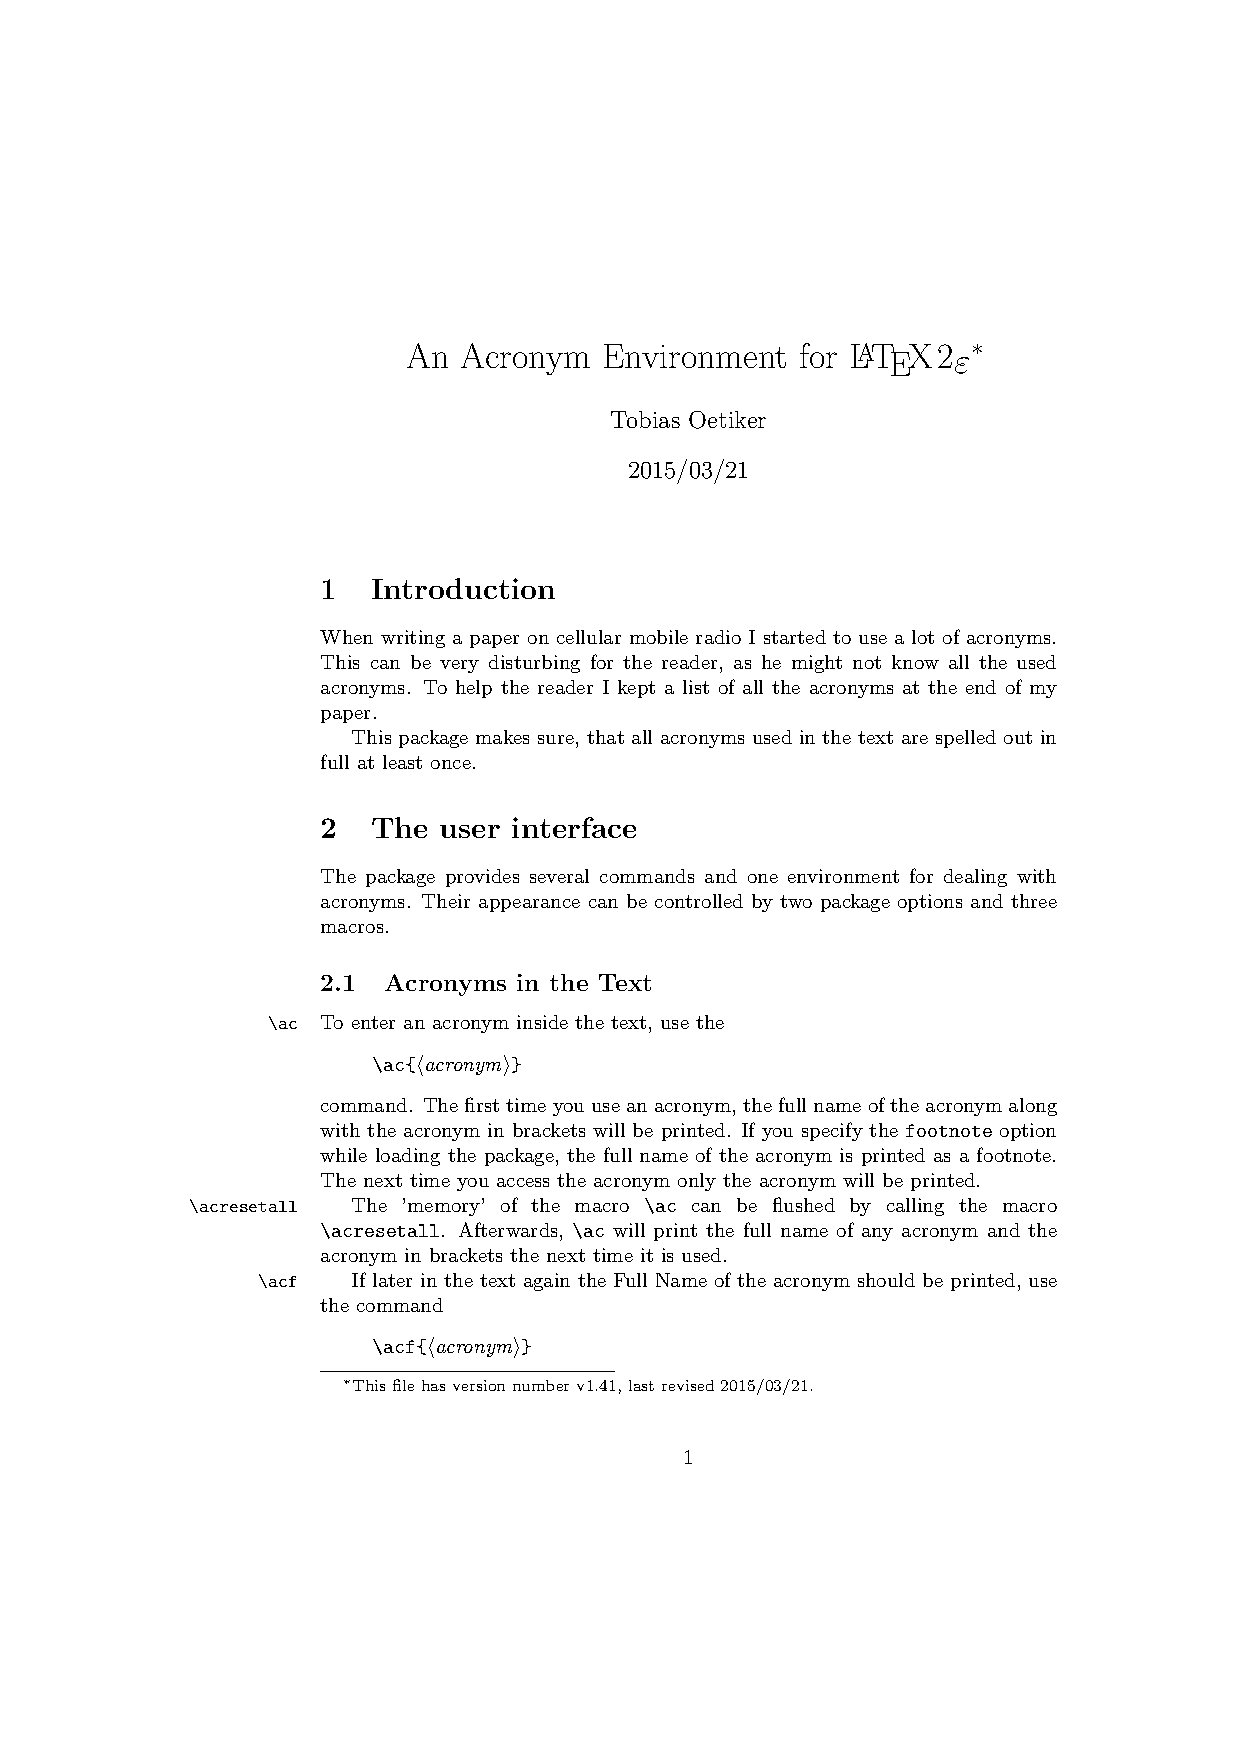
\includepdf[pages=1-3,frame=false,pagecommand={}]{anexos/acronym.pdf}


% ---
\chapter{Cras non urna sed feugiat cum sociis natoque penatibus}
% ---

\lipsum[1]



\end{anexosenv}



%---------------------------------------------------------------------
% INDICE REMISSIVO - Quando necessário 
% As palavras indexadas devem ser definidas com \index{} no texto
%---------------------------------------------------------------------
\phantompart
\printindex
%\todonum[inline]{remover indice remissivo se não for necessário}

%---------------------------------------------------------------------

\end{document}